\documentclass{beamer}

\mode<presentation>
{
  \usetheme{Warsaw}
  %\usecolortheme{crane}
  % or ...

  \setbeamercovered{transparent}
  % or whatever (possibly just delete it)
}

% Pacotes de linguas e fontes
\usepackage[portuguese]{nomencl}
\usepackage[english]{babel}
\usepackage[latin1]{inputenc}
\usepackage{times}
\usepackage[T1]{fontenc}
\usepackage{colortbl}
\usepackage{algorithm2e}

% Or whatever. Note that the encoding and the font should match. If T1
% does not look nice, try deleting the line with the fontenc.


\title[F�nix Firewall System] % (optional, use only with long paper titles)
{F�nix Firewall System}

\subtitle
{Um Firewall Pessoal Sens�vel ao Contexto para Dispositivos M�veis}

\author[Marcos Alves T. de Azevedo] % (optional, use only with lots of authors)
{Marcos Alves T. de Azevedo}
% - Give the names in the same order as the appear in the paper.
% - Use the \inst{?} command only if the authors have different
%   affiliation.

\institute[Universidade Federal de Goi�s] % (optional, but mostly needed)
{
  Instituto de Inform�tica\\
  Universidade Federal de Goi�s  
}
% - Use the \inst command only if there are several affiliations.
% - Keep it simple, no one is interested in your street address.

\date[Julho 2008] % (optional, should be abbreviation of conference name)
{Defesa de disserta��o de mestrado, 2008}
% - Either use conference name or its abbreviation.
% - Not really informative to the audience, more for people (including
%   yourself) who are reading the slides online

\subject{F�nix Firewall System}
% This is only inserted into the PDF information catalog. Can be left
% out. 

% If you have a file called "university-logo-filename.xxx", where xxx
% is a graphic format that can be processed by latex or pdflatex,
% resp., then you can add a logo as follows:

% \pgfdeclareimage[height=0.5cm]{Fenix_Picture}{Fenix_Picture}
% \logo{\pgfuseimage{Fenix_Picture}}

% Delete this, if you do not want the table of contents to pop up at
% the beginning of each subsection:
%\AtBeginSubsection[]
%{
% \begin{frame}<beamer>[allowframebreaks]
%    \frametitle{Agenda}
%    \tableofcontents[currentsection,currentsubsection]
%  \end{frame}
%}

% If you wish to uncover everything in a step-wise fashion, uncomment
% the following command: 
\beamerdefaultoverlayspecification{<+->}

\begin{document}

\begin{frame}
  \titlepage
\end{frame}

\begin{frame}[allowframebreaks]
  \frametitle{Agenda}
  \tableofcontents %[pausesections]
  % You might wish to add the option [pausesections]
\end{frame}

%=========================================================================
\beamerdefaultoverlayspecification{<*>}

% Inclusao das secoes
\section{Introdu��o}

\begin{frame}
\frametitle{\alert{Pr�ximos Slides}}
	\beamerdefaultoverlayspecification{<+->}
	
		\begin{enumerate}
			\item Introdu��o
			\item Motiva��o
			\item Justificativa
			\item Objetivos do Trabalho
		\end{enumerate}

	\beamerdefaultoverlayspecification{<*>}
\end{frame}

\subsection{Motiva��o}

\begin{frame}
  \frametitle{Motiva��o}

		\begin{itemize}
		  \item Engenhosidade e n�mero crescente das amea�as virtuais.\\
			  		Pesquisas dizem que \textbf{83\% das operadoras} de telefonia m�vel no mundo foram v�timas de ataques em seus dispositivos.
			\item Entre os anos de \textbf{2007} para \textbf{2008} surgiram \textbf{350 tipos de malwares} diferentes para dispositivos m�veis.
		\end{itemize}
			
\end{frame}

\begin{frame}
  \frametitle{Motiva��o}
  \framesubtitle{10\textsuperscript{\d a} Pesquisa realizada em 2007 pela M�dulo Security.}

			\begin{figure}[htbp]
				\centering
					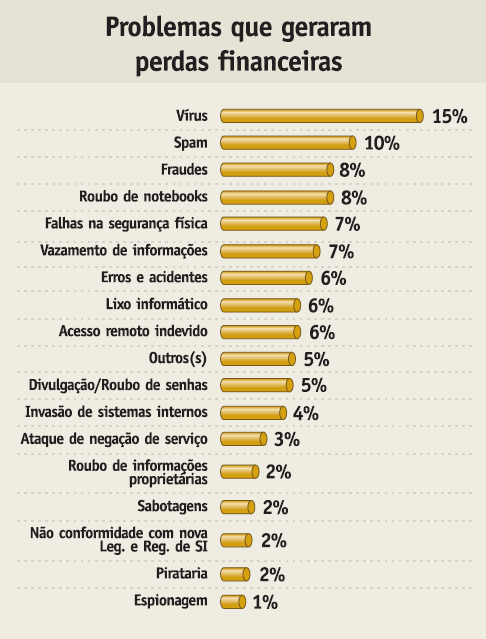
\includegraphics[width=0.40\textwidth]{../Pictures/Baixa/Estatistica_Problemas.png}
				\label{fig:Estatistica_Problemas}
			\end{figure}

\end{frame}


%_______________________________________________________________________
\subsection{Justificativa}


\begin{frame}
  \frametitle{Motiva��o}

			\begin{figure}[htbp]
				\centering
					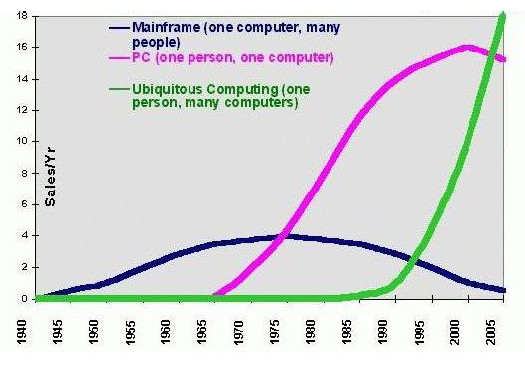
\includegraphics[width=0.80\textwidth]{../Pictures/Baixa/Grafico_Weiser.png}
				\label{fig:Grafico_Weiser}
			\end{figure}

\end{frame}

\begin{frame}
  \frametitle{Porque usar um Firewall?}
  
	\begin{center} 
			\LARGE \textbf{Conectar-se � Internet sem um \alert{Firewall} � como deixar as chaves do carro no contato, o motor ligado e as portas destravadas enquanto voc� vai �s compras !}
	\end{center}

\end{frame}


\begin{frame}[allowframebreaks]
  \frametitle{Porque usar um Firewall?}	

		\begin{itemize}
			\item \textbf{Quanto tempo seu \alert{Dispositivo M�vel} passa completamente \alert{DESLIGADO} ?!}
			% \item	A mobilidade pode se tornar um grande problema de seguran�a!
			\item Redes wireless abertas tem se tornado cada vez mais comum.			
			\item	Dispositivos M�veis possuem uma variedade maior de interfaces de comunica��o:			
					\begin{enumerate}
						\item Bluetooth;
						\item Wi-Fi;
						\item USB;
						\item EDGE;
						\item GPRS;
						\item Infra-vermelho 
					\end{enumerate}					
		\end{itemize}

\end{frame}


\begin{frame}
  \frametitle{Porque usar um Firewall?}				
				
	\begin{itemize}
			\item Imagine um Cavalo de Tr�ia que foi instalado junto com aquele seu toque predileto que voc� baixou da internet, e este Trojan envia suas senhas enquanto voc� acessa \alert{E-mail e Internet Banking} do seu Dispositivo M�vel.			
			\item Imagine que o simples fato de acessar um site atrav�s de seu Dispositivo M�vel cause o \textbf{apagamento} de todos os seus dados pessoais (Agenda, Compromissos etc)...
	\end{itemize}

\end{frame}


\begin{frame}
  \frametitle{Porque usar um Firewall?}
			\begin{itemize}
				\item Imagine voc� esquecer o \textbf{Bluetooth} ligado e outras pessoas acessar seus dados pessoais.
				\item Imagine um Worm como o \textbf{Blaster} para Dispositivos M�veis, que cause uma \textbf{Nega��o} nos servi�os de Telefonia m�vel...
								
			\end{itemize}
\end{frame}

				
\begin{frame}
  \frametitle{Porque usar um Firewall?}

			\begin{itemize}
				\item \alert{Sem} um Firewall voc� est� sujeito a v�rios ataques:
						\begin{enumerate}
							\item V�rus;
							\item Worms;
							\item Cavalos de Tr�ia;
							\item SynFlood;
							\item Ping of Death;
							\item Smurf;							
							\item Outros...
						\end{enumerate} 			
			\end{itemize}		
  
\end{frame}


%_______________________________________________________________________
\subsection{Objetivos do Trabalho}
\begin{frame}
  \frametitle{Objetivos do Trabalho?}

	\begin{figure}[htbp]
			\centering
				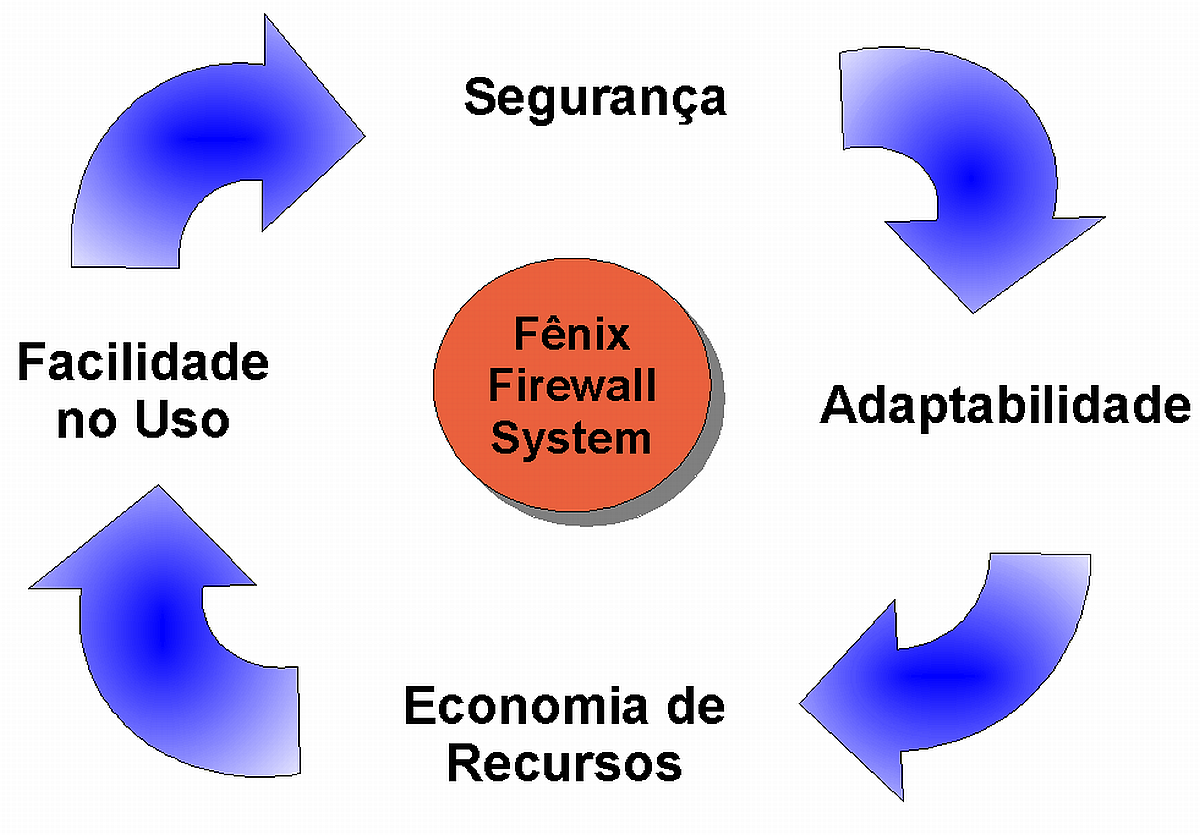
\includegraphics[width=0.80\textwidth]{../Pictures/Baixa/Ciclo_Fenix.png}
				\label{fig:Ciclo_Fenix}
			\end{figure}

\end{frame}
\section{F�nix Firewall System}

\begin{frame}
  \frametitle{Conhecendo a F�nix}
  
			\begin{figure}[htbp]
				\centering
					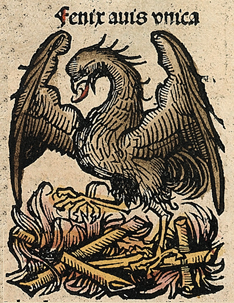
\includegraphics[width=0.40\textwidth]{../Pictures/Baixa/Fenix_Picture.png}				
				\label{fig:Fenix_Picture}
			\end{figure}

\end{frame}

\begin{frame}
\frametitle{\alert{Pr�ximos Slides}}
			
			\begin{center}
					\huge \textbf{Vis�o Geral da Arquitetura}.
			\end{center}
			
\end{frame}

%_______________________________________________________________________
\subsection{Vis�o Geral da Arquitetura}

\begin{frame}
  \frametitle{Vis�o Geral da Arquitetura}
  \framesubtitle{Do que o F�nix � capaz?}

			\begin{itemize}
				\item \alert{Controlar} o acesso ao dispositivo.
				\item \alert{Restringir} acessos entrantes e/ou saintes:
				
						\begin{enumerate}
							\item Dom�nios (Ex.: www.hackers.org);
							\item Redes  (Ex.: 10.0.0.0/8);	
							\item Sub-redes (Ex.: 200.137.197.129/27);
							\item Faixa de Endere�os IP (Ex.: 172.13.0.1 - 172.13.0.10);
							\item Endere�o IP (Ex.: 192.168.1.1/24)
						\end{enumerate}
						
				\item \alert{Notificar} quando conex�es suspeitas surgirem.
				\item \alert{Carregar} pol�ticas de seguran�a e prefer�ncias de usu�rio segundo a \textbf{localiza��o}.
				\item \alert{Sincronizar} e receber \alert{notifica��es} de seguran�a com uma Plataforma Distribu�da (\textbf{Opcional}).
			\end{itemize}

\end{frame}

\begin{frame}
	\frametitle{Ataques detectados pelo F�nix}
  
			\begin{itemize}
				\item Varreduras de portas.
				\item Worms e Cavalos de Tr�ia.
				\item Ataques DoS (tradicionais).
				\item IP Spoofing.
				\item Roteamento dirigido.
				\item Ping O'Death.
				\item SYN Flood.
				\item Ataques contra o protocolo NETBIOS.
				\item Ataques contra o X-Windows.				
				\item Ataque de Fragmenta��o.
				\item Varredura invis�vel.
				\item Transpar�ncia dos dados na rede.				
			\end{itemize}

\end{frame}



\begin{frame}
  \frametitle{Vis�o Geral da Arquitetura}

		\begin{block}{Arquitetura do F�nix Firewall}		
			\begin{enumerate}
				\item \alert{\textbf{Arquitetura Embarcada}}.\\
							Instalada no Dispositivo M�vel.
											
				\item \alert{\textbf{Arquitetura Distribu�da}}.\\
							Parte \textbf{Opcional}, que � instalada em computadores na WEB. Interessante para \textbf{Usu�rios Avan�ados} e \textbf{Terceiros}.
							
			\end{enumerate}
		\end{block}

\end{frame}


%_______________________________________________________________________

\subsection{Arquitetura Embarcada}

\begin{frame}
  \frametitle{\alert{Pr�ximos Slides}}
			
			\begin{center}
					\huge \textbf{Arquitetura Embarcada}.
			\end{center}
			
\end{frame}


\begin{frame}
  \frametitle{Arquitetura Embarcada}
  
\begin{figure}[htbp]
	\centering
		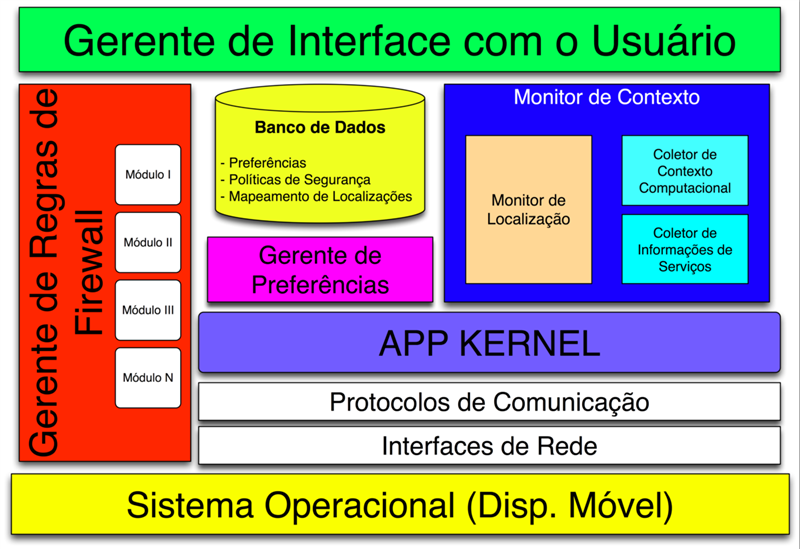
\includegraphics[width=0.80\textwidth]{../Pictures/Sequencias/Arquitetura_Embarcada/Arquitetura_Embarcada.png}
	\label{fig:Arquitetura_Embarcada}
\end{figure}
  
\end{frame}


\begin{frame}
  \frametitle{Arquitetura Embarcada}
  \framesubtitle{Sistema Operacional}
  
\begin{figure}[htbp]
	\centering
		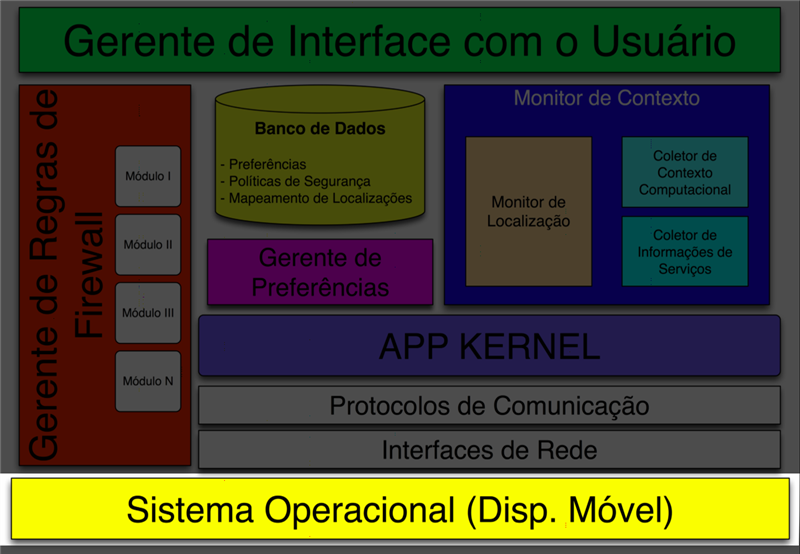
\includegraphics[width=0.80\textwidth]{../Pictures/Sequencias/Arquitetura_Embarcada/SistemaOperacional.png}
	\label{fig:SistemaOperacional}
\end{figure}
  
\end{frame}


\begin{frame}
  \frametitle{Arquitetura Embarcada}
  \framesubtitle{AppKernel \alert{(N�cleo)}}
  
\begin{figure}[htbp]
	\centering
		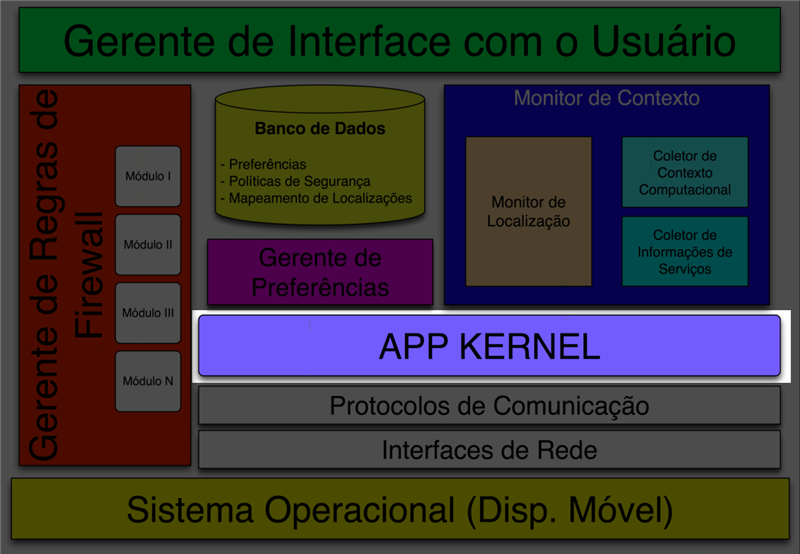
\includegraphics[width=0.80\textwidth]{../Pictures/Sequencias/Arquitetura_Embarcada/AppKernel.png}
	\label{fig:AppKernel}
\end{figure}
  
\end{frame}

\begin{frame}
  \frametitle{Arquitetura Embarcada}
  \framesubtitle{Gerente de Prefer�ncias}
  
\begin{figure}[htbp]
	\centering
		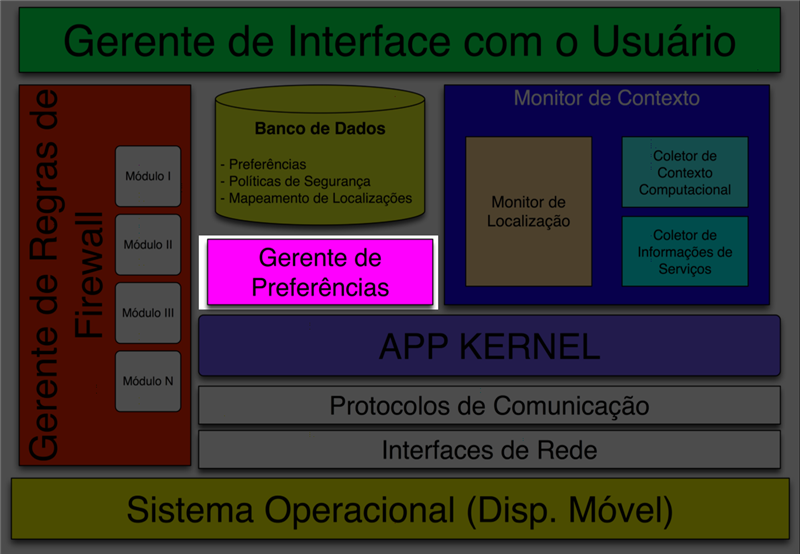
\includegraphics[width=0.80\textwidth]{../Pictures/Sequencias/Arquitetura_Embarcada/GerentePreferencias.png}
	\label{fig:GerentePreferencias}
\end{figure}
  
\end{frame}


\begin{frame}
  \frametitle{Arquitetura Embarcada}
	\framesubtitle{Banco de Dados}  
	
\begin{figure}[htbp]
	\centering
		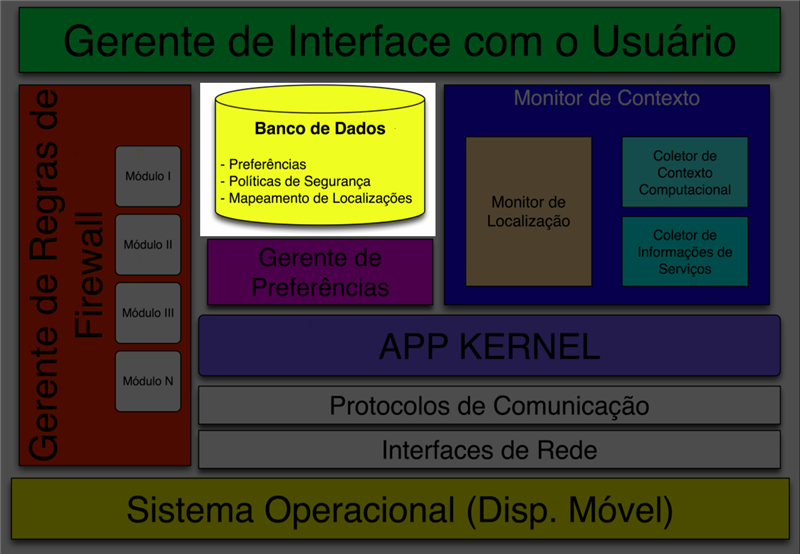
\includegraphics[width=0.80\textwidth]{../Pictures/Sequencias/Arquitetura_Embarcada/BancoDados.png}
	\label{fig:BancoDados}
\end{figure}
  
\end{frame}


\begin{frame}
  \frametitle{Arquitetura Embarcada}
  \framesubtitle{Gerente de Regras de Firewall}
  
\begin{figure}[htbp]
	\centering
		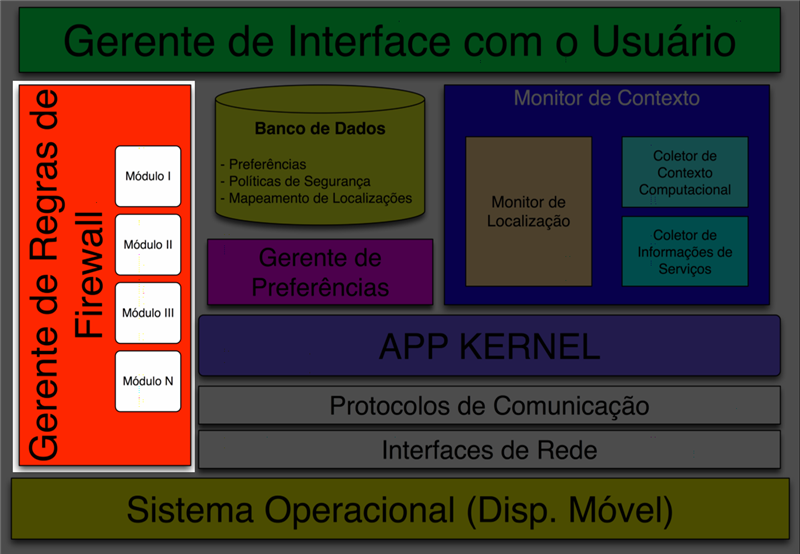
\includegraphics[width=0.80\textwidth]{../Pictures/Sequencias/Arquitetura_Embarcada/GerenteRegrasFirewall.png}
	\label{fig:GerenteRegrasFirewall}
\end{figure}
  
\end{frame}


\begin{frame}
  \frametitle{Arquitetura Embarcada}
  \framesubtitle{Monitor de Contexto}
  
\begin{figure}[htbp]
	\centering
		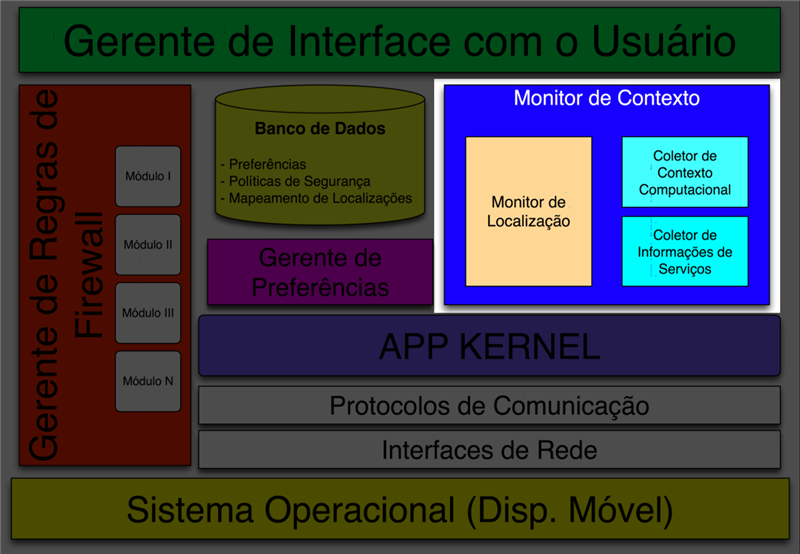
\includegraphics[width=0.80\textwidth]{../Pictures/Sequencias/Arquitetura_Embarcada/MonitorContexto.png}
	\label{fig:MonitorContexto}
\end{figure}
  
\end{frame}


\begin{frame}
  \frametitle{Arquitetura Embarcada}
  \framesubtitle{Monitor de Localiza��o}
  
\begin{figure}[htbp]
	\centering
		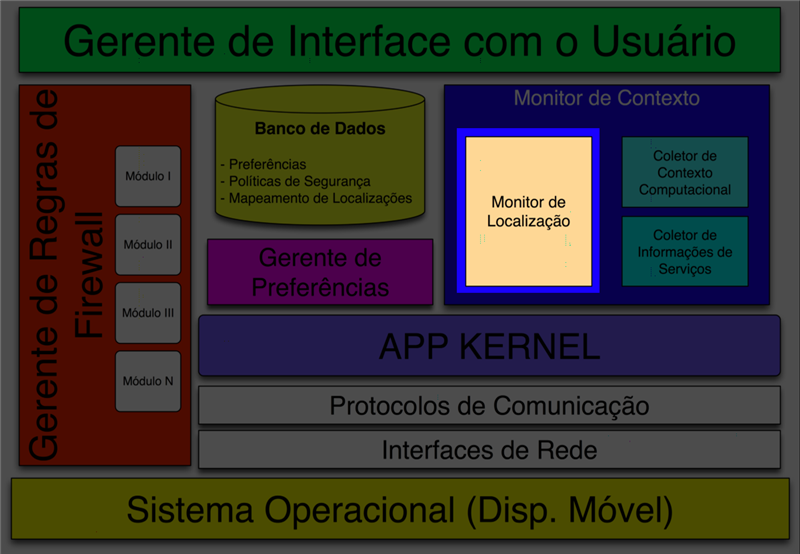
\includegraphics[width=0.80\textwidth]{../Pictures/Sequencias/Arquitetura_Embarcada/MonitorLocalizacao.png}
	\label{fig:MonitorLocalizacao}
\end{figure}
  
\end{frame}


\begin{frame}
  \frametitle{Arquitetura Embarcada}
  \framesubtitle{Coletor de Contexto Computacional}
  
\begin{figure}[htbp]
	\centering
		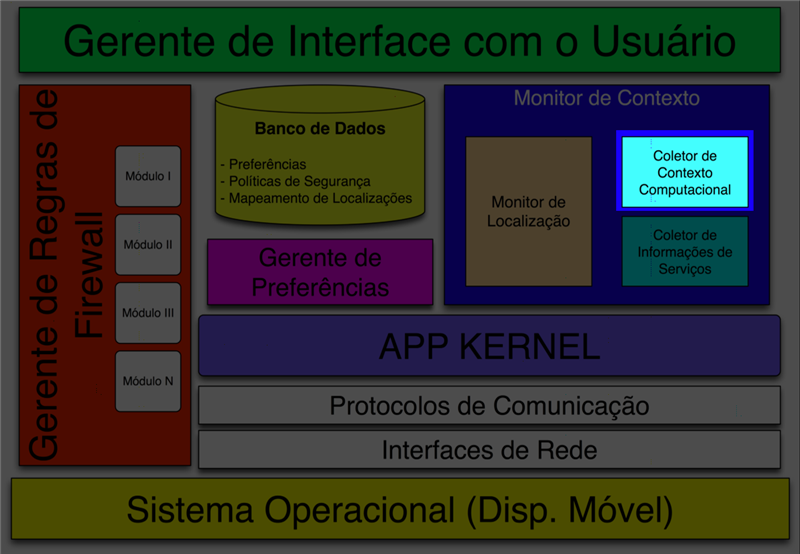
\includegraphics[width=0.80\textwidth]{../Pictures/Sequencias/Arquitetura_Embarcada/ColetorContextoComputacional.png}
	\label{fig:ColetorContextoComputacional}
\end{figure}
  
\end{frame}


\begin{frame}
  \frametitle{Arquitetura Embarcada}
  \framesubtitle{Coletor de Informa��es de Servi�os}
  
\begin{figure}[htbp]
	\centering
		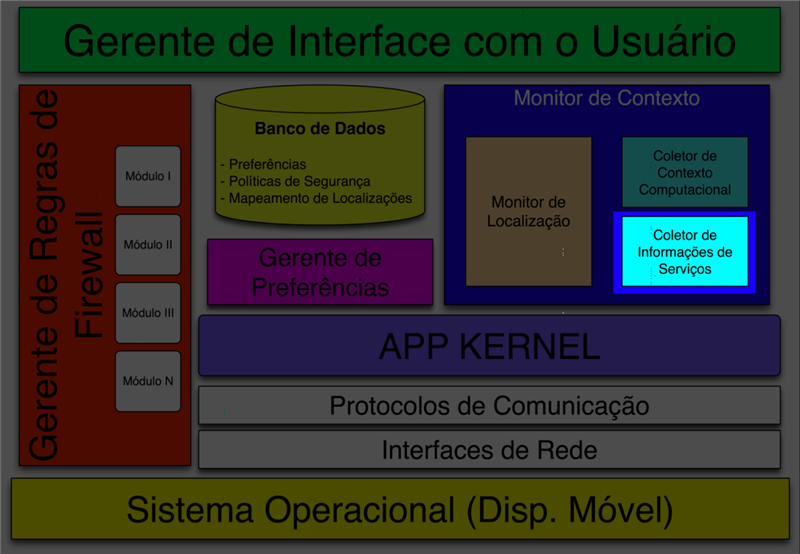
\includegraphics[width=0.80\textwidth]{../Pictures/Sequencias/Arquitetura_Embarcada/ColetorInformacoesServico.png}
	\label{fig:ColetorInformacoesServico}
\end{figure}
  
\end{frame}


\begin{frame}
  \frametitle{Arquitetura Embarcada}
  \framesubtitle{Gerente de Interfaces}
  
\begin{figure}[htbp]
	\centering
		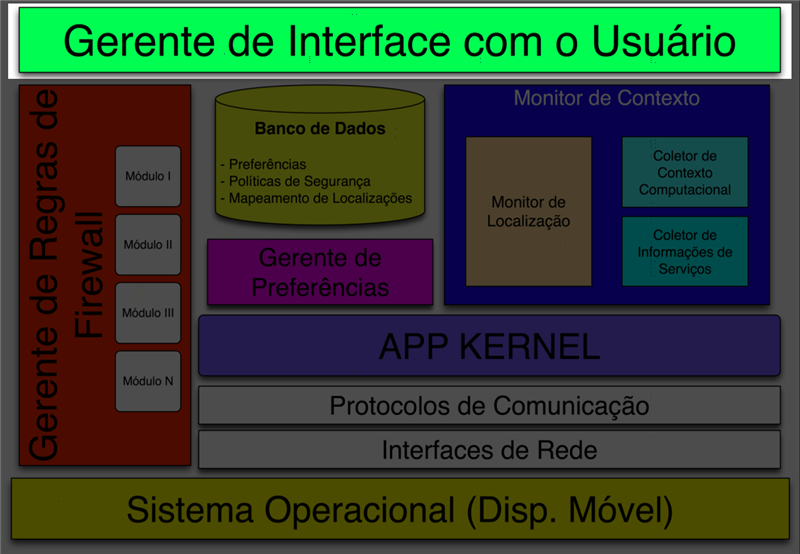
\includegraphics[width=0.80\textwidth]{../Pictures/Sequencias/Arquitetura_Embarcada/GerenteInterface.png}
	\label{fig:GerenteInterface}
\end{figure}
  
\end{frame}


\begin{frame}
  \frametitle{Arquitetura Embarcada}
  
\begin{figure}[htbp]
	\centering
		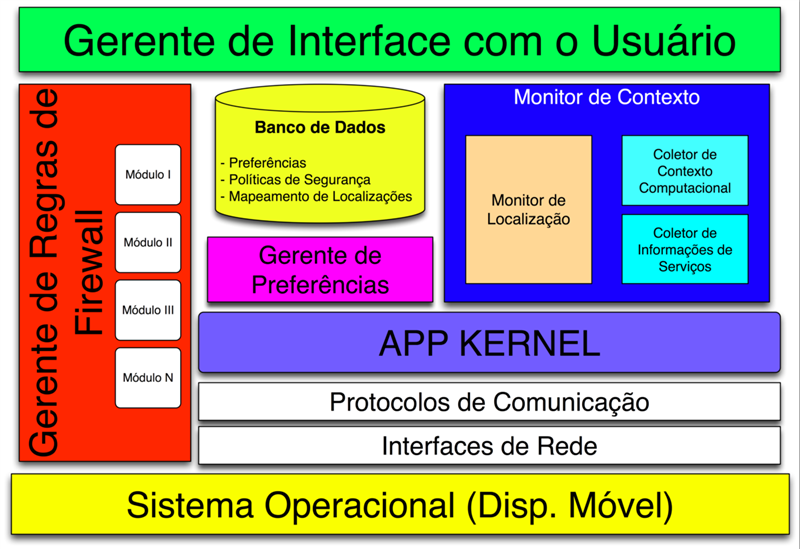
\includegraphics[width=0.80\textwidth]{../Pictures/Sequencias/Arquitetura_Embarcada/Arquitetura_Embarcada.png}
	\label{fig:Arquitetura_Embarcada}
\end{figure}
  
\end{frame}





%_______________________________________________________________________

\subsection{Arquitetura Distribu�da}

\begin{frame}
  \frametitle{\alert{Pr�ximos Slides}}
			
			\begin{center}
					\huge \textbf{Arquitetura Distribu�da}.
			\end{center}
			
\end{frame}

\begin{frame}
  \frametitle{Arquitetura Distribu�da}
  \framesubtitle{Vis�o Geral}
  
			\begin{figure}[htbp]
				\centering 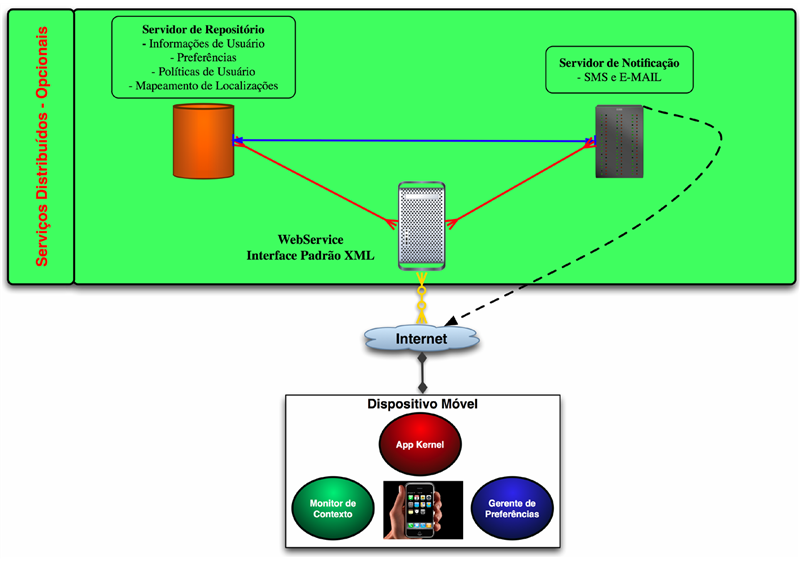
\includegraphics[width=0.80\textwidth]{../Pictures/Sequencias/Arquitetura_Distribuida/Arquitetura_Distribuida.png}
				\label{fig:Arquitetura_Distribuida}
			\end{figure}

\end{frame}


\begin{frame}[allowframebreaks]
		\frametitle{Plataforma Distribu�da (Uma \alert{\textbf{Op��o}} Inteligente)}
		
		
		\begin{block}{Controle de acesso gerenciado por grupos}
				\begin{enumerate}
						\item \alert{\textbf{Administradores}}
						\\ Grupo de usu�rios com acesso privilegiado respons�vel pela ger�ncia e manuten��o da plataforma distribu�da.
						\item \alert{\textbf{Usu�rios}}
						\\ Grupo de usu�rios ordin�rios com acesso restrito � plataforma distribu�da.
				\end{enumerate}			
		\end{block}
		
		\newpage		
		\begin{itemize}
			\item Facilita \alert{ger�ncia} dos dispositivos m�veis por \textbf{terceiros}.
			\item Permite maior \alert{integra��o} entre os dispositivos m�veis.
			\item Permite que o \alert{Administrador} envie notifica��es importantes aos usu�rios.
			\item Permite que o \alert{Administrador} insira uma nova pol�tica de seguran�a de forma autorit�ria, evitando ataques do tipo \textbf{0-day (Zero Day)}.								
			\item Permite que o usu�rio \textbf{troque de dispositivo} e mantenha as mesmas prefer�ncias e pol�ticas de seguran�a.			
		\end{itemize}
		
\end{frame}


\begin{frame}
  \frametitle{Arquitetura Distribu�da}
  \framesubtitle{Dispositivo M�vel}
  
\begin{figure}[htbp]
	\centering
		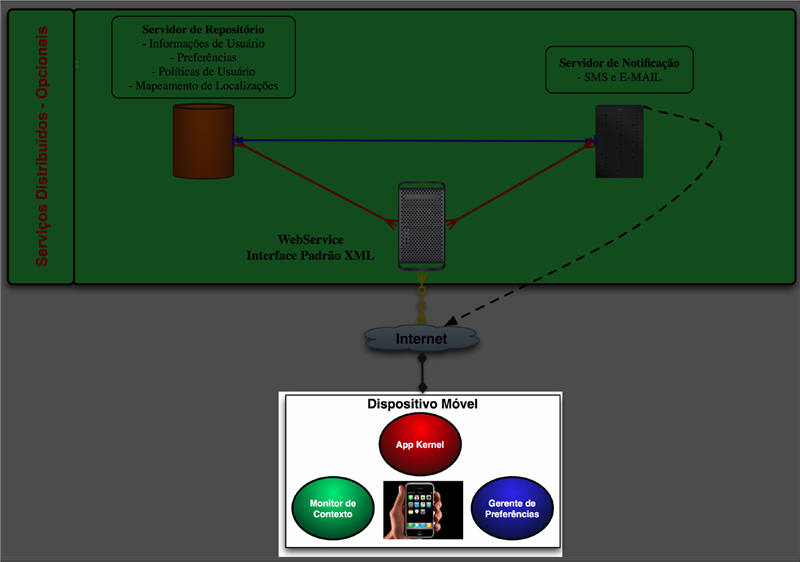
\includegraphics[width=0.80\textwidth]{../Pictures/Sequencias/Arquitetura_Distribuida/DispositivoMovel.png}
	\label{fig:DispositivoMovel}
\end{figure}

\end{frame}


\begin{frame}
  \frametitle{Arquitetura Distribu�da}
  \framesubtitle{Conex�o com a Internet}
  
\begin{figure}[htbp]
	\centering
		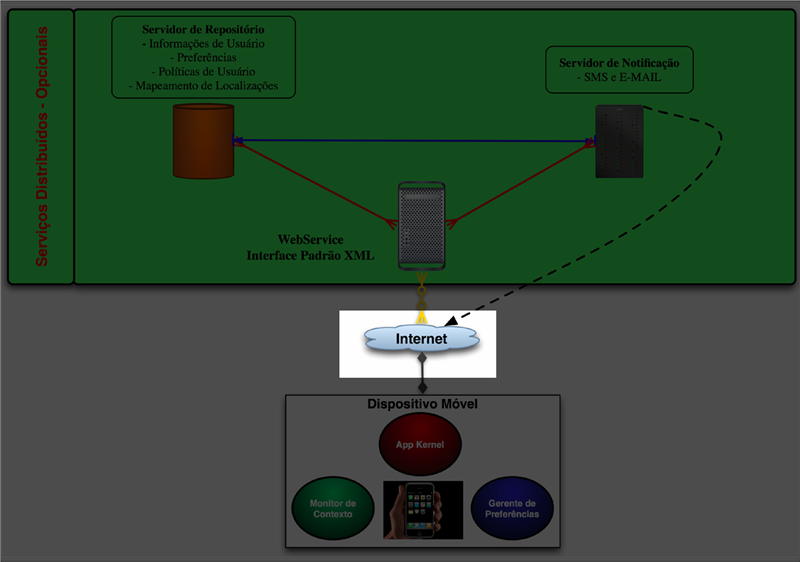
\includegraphics[width=0.80\textwidth]{../Pictures/Sequencias/Arquitetura_Distribuida/Internet.png}
	\label{fig:Internet}
\end{figure}

\end{frame}


\begin{frame}
  \frametitle{Arquitetura Distribu�da}
  \framesubtitle{Servidor WebService}
  
\begin{figure}[htbp]
	\centering
		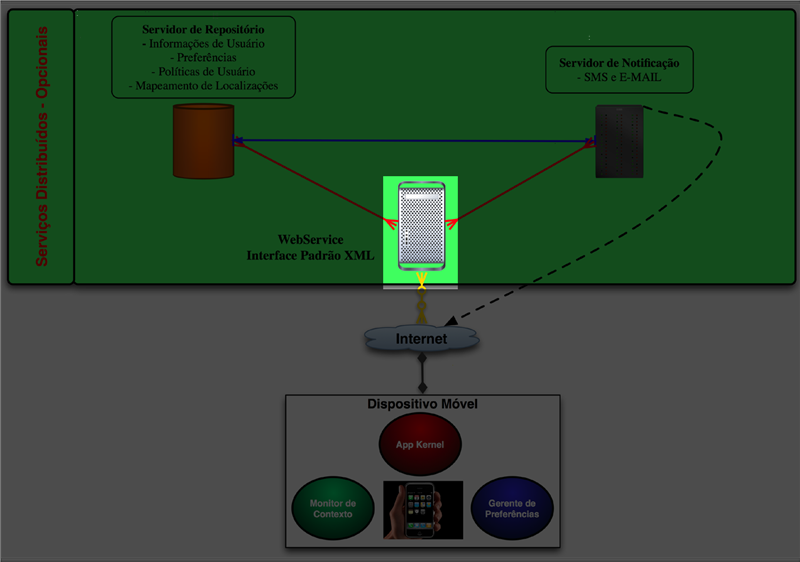
\includegraphics[width=0.80\textwidth]{../Pictures/Sequencias/Arquitetura_Distribuida/WebService.png}
	\label{fig:WebService}
\end{figure}

\end{frame}

\begin{frame}
  \frametitle{Arquitetura Distribu�da}
  \framesubtitle{Conex�o Disp. M�vel com Serv. WebService}
  
\begin{figure}[htbp]
	\centering
		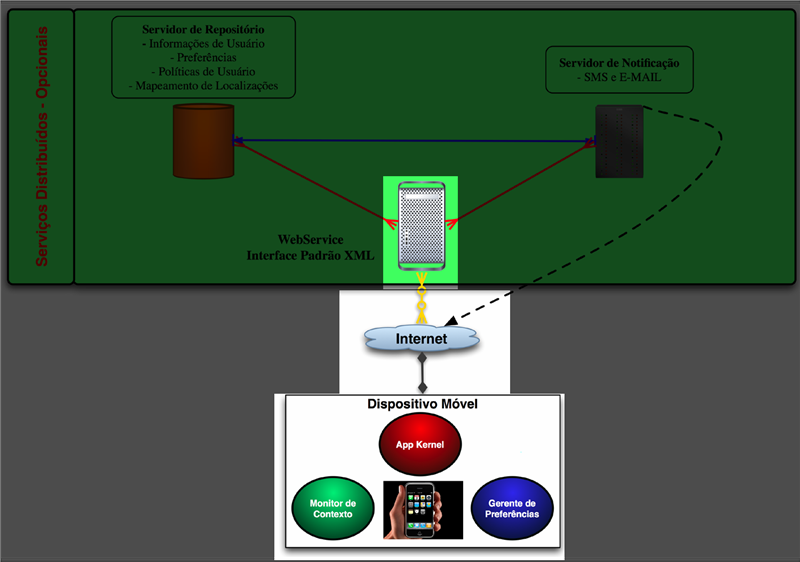
\includegraphics[width=0.80\textwidth]{../Pictures/Sequencias/Arquitetura_Distribuida/Conexao_Movel_WebService.png}
	\label{fig:ConexaoWebService}
\end{figure}

\end{frame}


\begin{frame}
  \frametitle{Arquitetura Distribu�da}
  \framesubtitle{Servidor de Reposit�rio}
  
\begin{figure}[htbp]
	\centering
		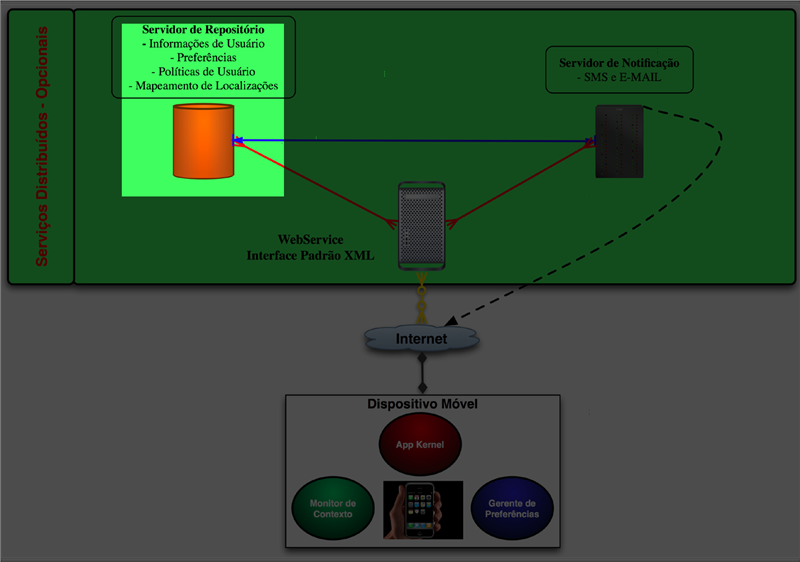
\includegraphics[width=0.80\textwidth]{../Pictures/Sequencias/Arquitetura_Distribuida/ServidorRepositorio.png}
	\label{fig:ServidorRepositorio}
\end{figure}

\end{frame}


\begin{frame}
  \frametitle{Arquitetura Distribu�da}
  \framesubtitle{Servidor de Notifica��es}
  
\begin{figure}[htbp]
	\centering
		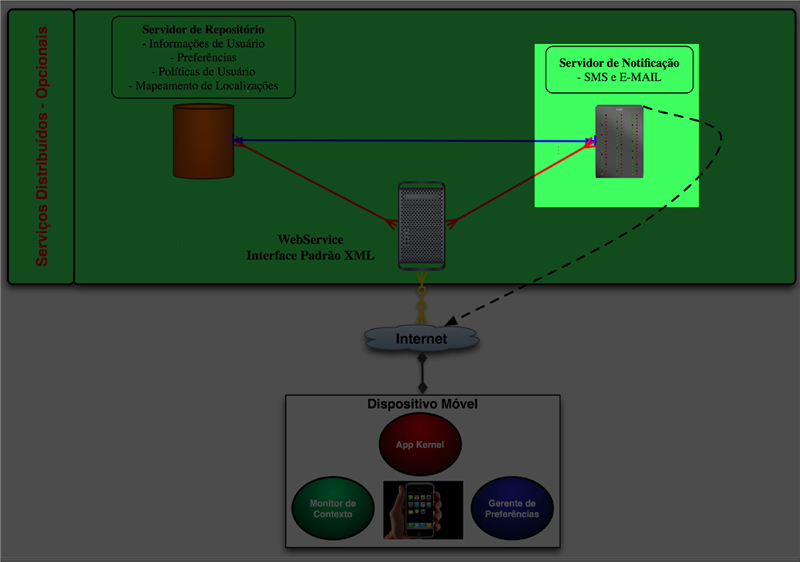
\includegraphics[width=0.80\textwidth]{../Pictures/Sequencias/Arquitetura_Distribuida/ServidorNotificacao.png}
	\label{fig:ServidorNotificacao}
\end{figure}

\end{frame}


\begin{frame}
  \frametitle{Arquitetura Distribu�da}
  \framesubtitle{Comunica��o \alert{entre os Servidores}}

\begin{figure}[htbp]
	\centering
		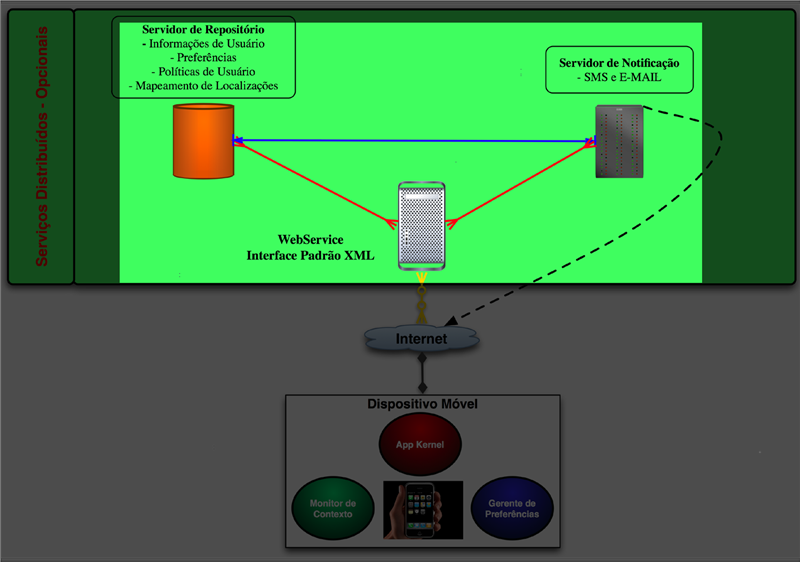
\includegraphics[width=0.80\textwidth]{../Pictures/Sequencias/Arquitetura_Distribuida/Conexao_Servidores.png}
	\label{fig:Conexao_Servidores}
\end{figure}

\end{frame}


\begin{frame}
  \frametitle{Arquitetura Distribu�da}
  \framesubtitle{Comunica��o entre \alert{Servidor WebService} e \alert{Servidor Reposit�rio}}
  
\begin{figure}[htbp]
	\centering
		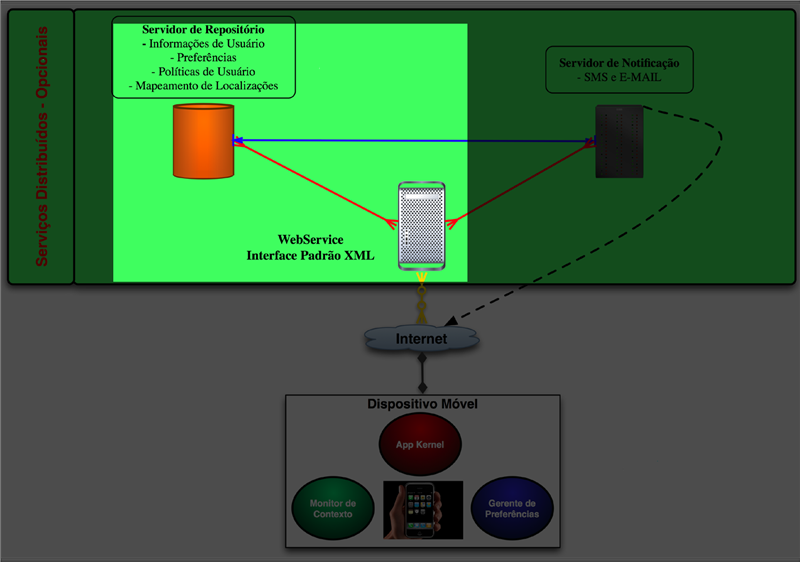
\includegraphics[width=0.80\textwidth]{../Pictures/Sequencias/Arquitetura_Distribuida/Conexao_WebService_BancoDados.png}
	\label{fig:Conexao_WebService_BancoDados}
\end{figure}

\end{frame}


\begin{frame}
  \frametitle{Arquitetura Distribu�da}
  \framesubtitle{Comunica��o entre \alert{Servidor WebService} e \alert{Servidor Notifica��o}}
  
\begin{figure}[htbp]
	\centering		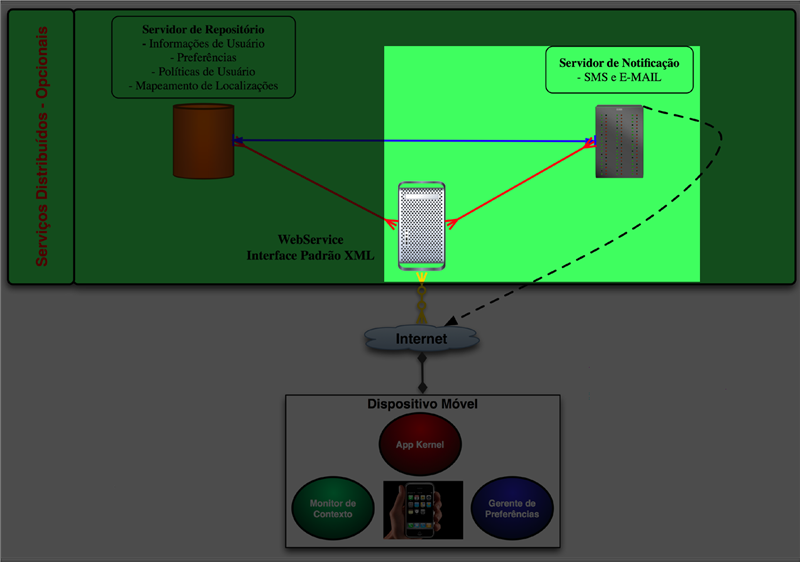
\includegraphics[width=0.80\textwidth]{../Pictures/Sequencias/Arquitetura_Distribuida/Conexao_WebService_Notificacao.png}
	\label{fig:Conexao_WebService_Notificacao}
\end{figure}

\end{frame}


\begin{frame}
  \frametitle{Arquitetura Distribu�da}
  \framesubtitle{Comunica��o entre \alert{Servidor Notifica��o} e \alert{Dispositivo M�vel}}
  
\begin{figure}[htbp]
	\centering
		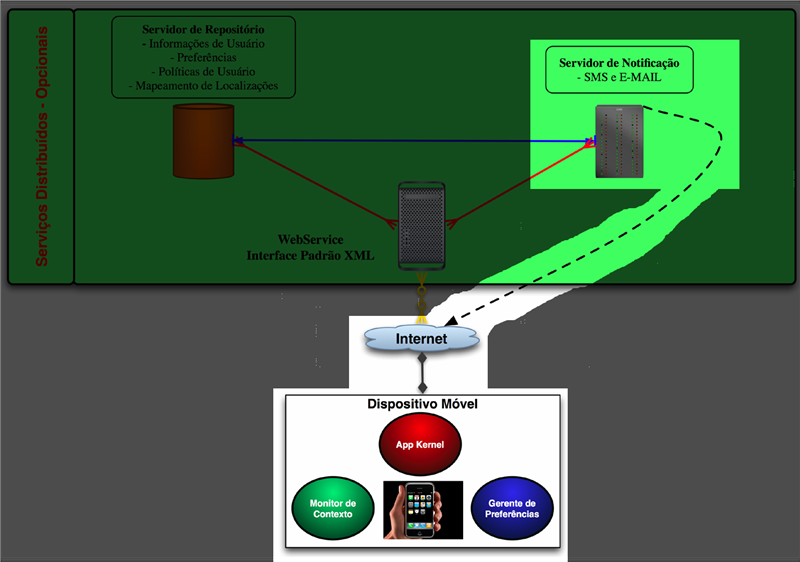
\includegraphics[width=0.80\textwidth]{../Pictures/Sequencias/Arquitetura_Distribuida/Conexao_Notificacao_Movel.png}
	\label{fig:Conexao_Notificacao_Movel}
\end{figure}

\end{frame}


\begin{frame}
  \frametitle{Arquitetura Distribu�da}
  \framesubtitle{Vis�o Geral}
  
\begin{figure}[htbp]
	\centering
		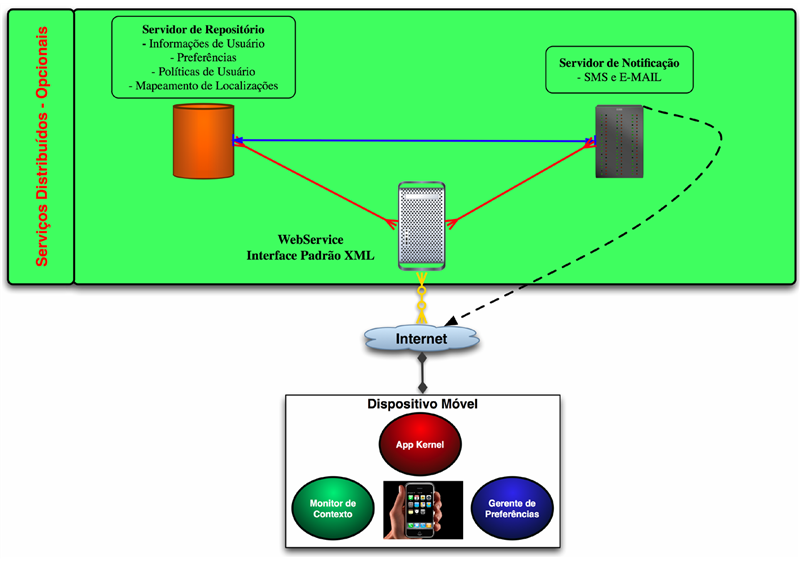
\includegraphics[width=0.80\textwidth]{../Pictures/Sequencias/Arquitetura_Distribuida/Arquitetura_Distribuida.png}
	\label{fig:Arquitetura_Distribuida}
\end{figure}

\end{frame}



%_______________________________________________________________________

\subsection{Pol�tica de Seguran�a Baseada em Localiza��o}

\begin{frame}
\frametitle{\alert{Pr�ximos Slides}}
  
  \textbf{Implementa��o da Pol�tica de Seguran�a Baseada em Localiza��o}.
	
	\beamerdefaultoverlayspecification{<+->}
	\begin{itemize}
		\item Identificar a Localiza��o do Usu�rio.
		\item Mapear �reas.
		\item Carregar Pol�ticas de Seguran�a Baseada na Localiza��o do Usu�rio.
	\end{itemize}
	\beamerdefaultoverlayspecification{<*>}
	
\end{frame}


\begin{frame}
		\begin{center}
			\huge \textbf{Identificar uma Localiza��o}.
		\end{center}
\end{frame}


\begin{frame}
  \frametitle{Identificar uma Localiza��o}
  \framesubtitle{Sele��o Manual}
  
				\begin{itemize}
						\item \textbf{Forma Padr�o:}
								\begin{enumerate}
									\item Selecionar manualmente a Localiza��o.
								\end{enumerate}
				\end{itemize}
								
				\begin{figure}[htbp]
						\centering
						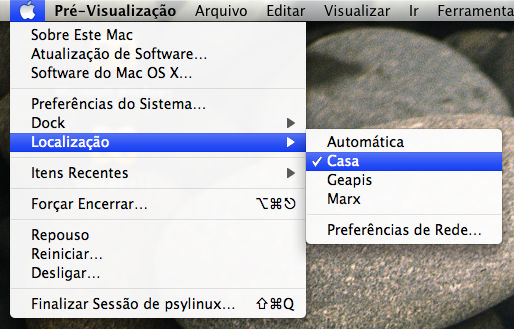
\includegraphics[width=0.60\textwidth]{../Pictures/Baixa/SelecaoManual.png}
						\label{fig:SelecaoManual}
				\end{figure}

\end{frame}


\begin{frame}
  \frametitle{Identificar uma Localiza��o}
  \framesubtitle{Sele��o Autom�tica \alert{(Opcional)}}								
			
	\begin{block}{Modos de Opera��o}
		\begin{enumerate}
				\item \alert{\textbf{Ambientes Outdoor:}}
						\begin{itemize}
								\item Usando o recurso \textbf{GPS} presente no dispositivo, caso exista.
						\end{itemize}	
		
				\item \alert{\textbf{Ambientes Indoor:}}
						\begin{itemize}
								\item Usando os recursos de \textbf{Localiza��o} oferecido pela \textbf{Arquitetura Distribu�da}.
						\end{itemize}
		\end{enumerate}
	\end{block}
								
\end{frame}


\begin{frame}
  \frametitle{\alert{GPS:} Identificar uma Localiza��o.}

			\begin{algorithm}[H]
				\SetLine	
				\textbf{Consulta} GPS \\
				$Local \longleftarrow raiz[ (x2{}-x1)\textsuperscript{\d 2} + (y2{}-y1)\textsuperscript{\d 2} ]$\;	
				\SetLine
				\Se	{$Local \subseteq banco.mapeamentos$}{
							\textbf{Selecione} $banco.mapeamento$\;
							\textbf{Carregue} $banco.politicas[Local]$\;
							\textbf{Carregue} $banco.preferencias[Local]$;				
				}
			\end{algorithm}

\end{frame}


\begin{frame}
\frametitle{\alert{Pr�ximos Slides}}

		\begin{center}
			\huge \textbf{Mapear uma �rea}.
		\end{center}
		
\end{frame}


\begin{frame}
  \frametitle{Mapear uma �rea (Introdu��o)}  
	
		\textbf{Discutiremos agora as abordagens de mapeamento relacionada aos t�picos abaixo:}
	
		\beamerdefaultoverlayspecification{<+->}
		\begin{itemize}
			\item Tipos de Mapeamento:
					\begin{enumerate}
						\item Indoor.
						\item Outdoor.
					\end{enumerate}
			\item O que � um mapeamento.
			\item Formas de mapeamento.
		\end{itemize}
		\beamerdefaultoverlayspecification{<*>} 
		 
\end{frame}


\begin{frame}
  \frametitle{Mapear uma �rea}
			
			\begin{itemize}
					\item Com a plataforma distribu�da o grupo \alert{Administrador} � capaz de mapear �reas comuns aos usu�rios.	
			\end{itemize}

			\begin{block}{Tipos de Mapeamento}					
					\begin{enumerate}
							\item As �reas comuns s�o definidas \textbf{exclusivamente} pelos administradores, e poder�o ser utilizadas por todos os usu�rios, \textit{ex.: Laborat�rio de Redes, Secretaria, Almoxarifado.}
				
							\item As �reas pessoais ser�o mapeadas pelo pr�prio usu�rio, e as mesmas n�o s�o vis�veis ou compartilhadas para os outros usu�rios  da plataforma.
					\end{enumerate}
  		\end{block}
\end{frame}


\begin{frame}
  \frametitle{Pol�tica de Seguran�a Baseada em Localiza��o}

  			\begin{figure}
					\centering
						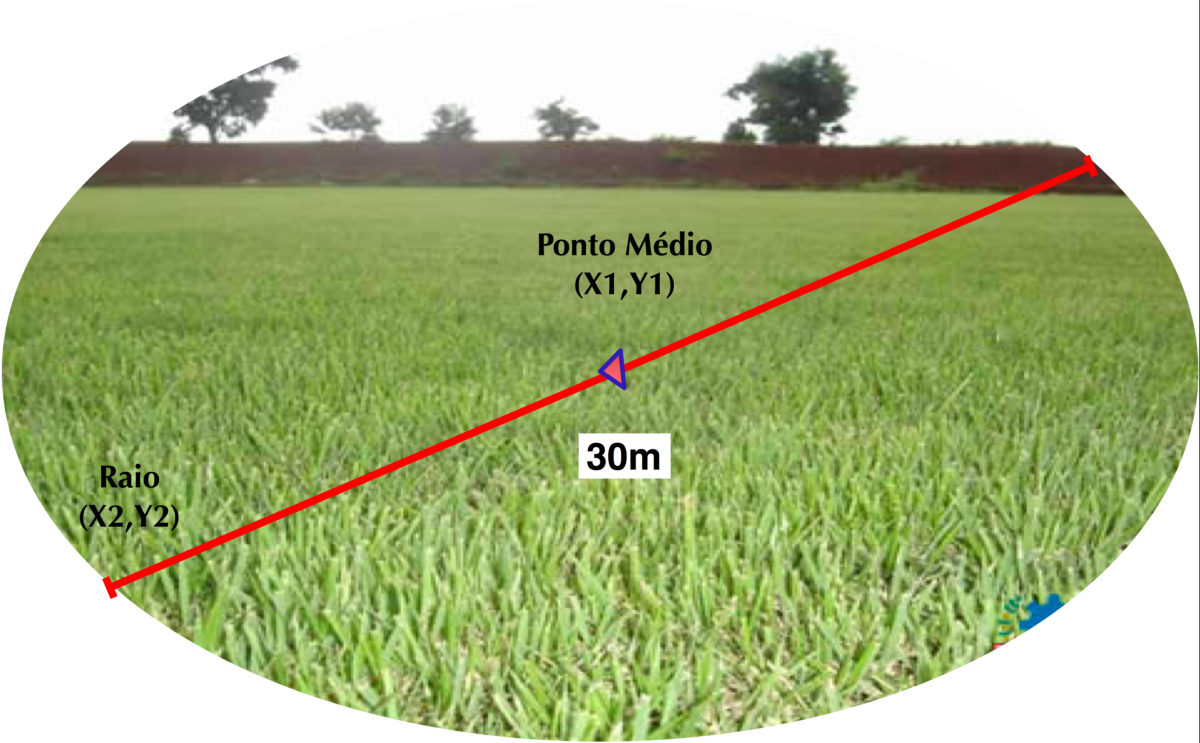
\includegraphics[width=0.90\textwidth]{../Pictures/Baixa/AlgoritmoGPS.png}
					\label{fig:AlgoritmoGPS}
				\end{figure}
				  
\end{frame}


\begin{frame}
  \frametitle{\alert{GPS:} Mapear uma �rea}

			\begin{algorithm}[H]
				\SetLine	
				\textbf{Consulta} GPS \\
				$Local \longleftarrow raiz[ (x2{}-x1)\textsuperscript{\d 2} + (y2{}-y1)\textsuperscript{\d 2} ]$\;	
				\SetLine
				\Se	{\textbf{n�o} ($Local \subseteq banco.mapeamentos$)}{			
						$distancia \longleftarrow raiz[(x1 {}- x2)2 + (y1 {}- y2)2]$\;
						$centro \longleftarrow distancia / 2$\;
						$area \longleftarrow 2 x Pi x (centro)2$\; 
						\textbf{Escreve} Entre com a Identifica��o para esta localiza��o\;
						\textbf{Salva} $Local$;
				}
			\end{algorithm}

\end{frame}

 
\begin{frame}
  \frametitle{Pol�tica de Seguran�a Baseada em Localiza��o}

   \begin{figure}[htb]
       \centering  % figura centralizada
       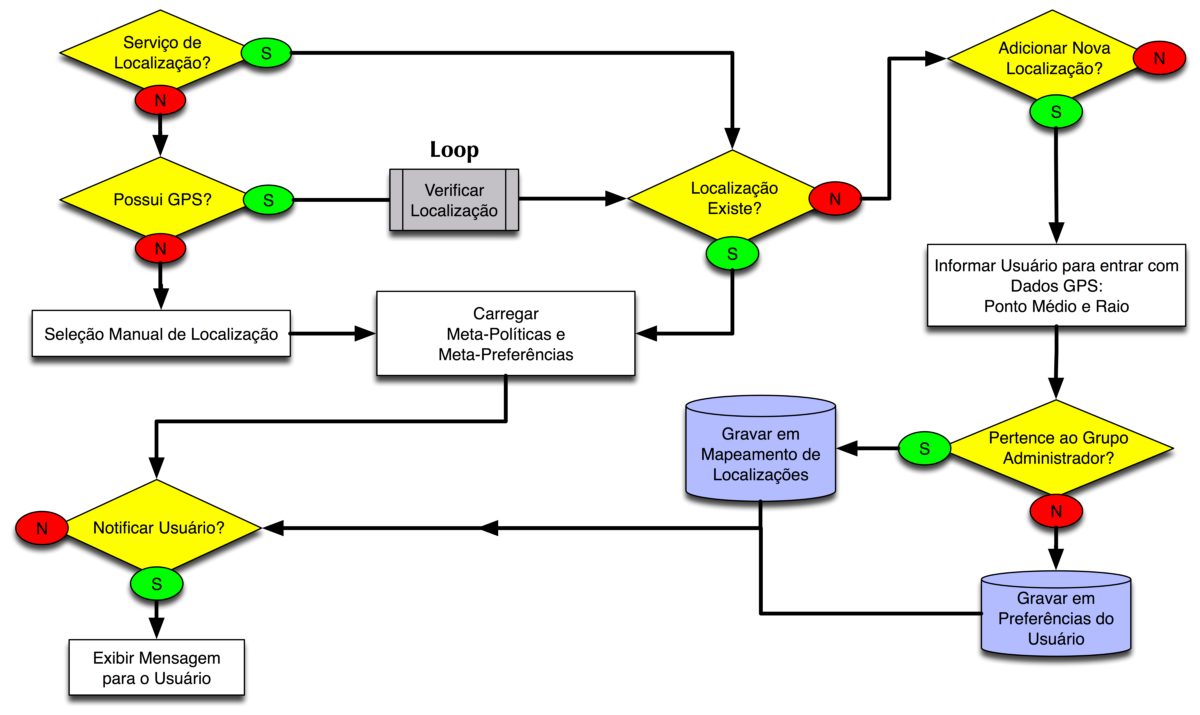
\includegraphics[width=0.90\textwidth]{../Pictures/Baixa/Fluxograma.png}
       \label{fig:Fluxograma}
   \end{figure}

\end{frame}


%_______________________________________________________________________

\subsection{Ilustrando o Funcionamento}

\begin{frame}
\frametitle{\alert{Pr�ximos Slides}}

		\begin{center}
			\huge \textbf{Ilustrando o Funcionamento}.
		\end{center}
		
\end{frame}


%%%%%%%%%%%%%%%%%%%%%%%%%%%%%%%%%%%%%%%%%%%%%%%%%%%%%%%%%%%%%%%%%%%%%%%%%%%%%%%%%%%%%%%
%% Cen�rio 1 - Carregando Meta-Pol�ticas e Meta-Prefer�ncias
%%%%%%%%%%%%%%%%%%%%%%%%%%%%%%%%%%%%%%%%%%%%%%%%%%%%%%%%%%%%%%%%%%%%%%%%%%%%%%%%%%%%%%%
\begin{frame}
  \frametitle{\textbf Dispositivo M�vel \alert{com} GPS}
  \framesubtitle{Carregando Meta-Pol�ticas e Meta-Prefer�ncias}

\begin{figure}[htbp]
	\centering
		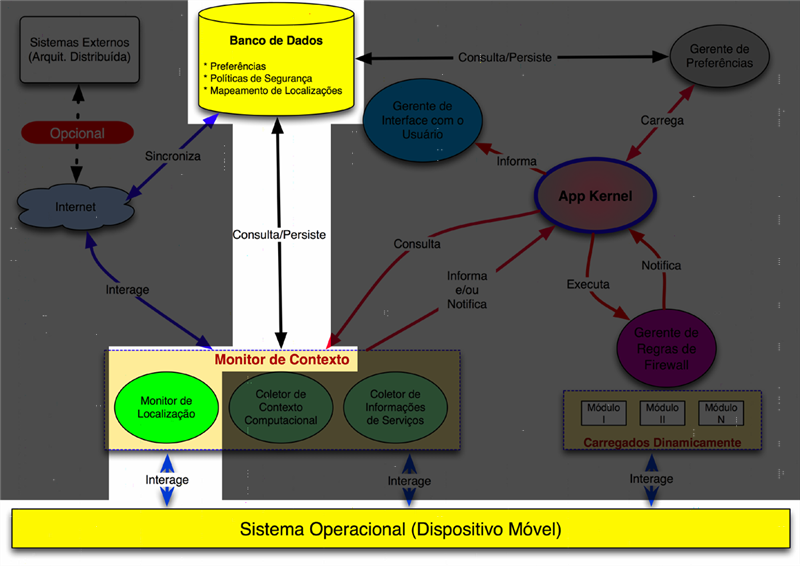
\includegraphics[width=0.80\textwidth]{../Pictures/Sequencias/Cenarios/CarregandoMetaDados_GPS/c1-1.png}
	\label{fig:c1-1}
\end{figure}

\end{frame}

\begin{frame}
  \frametitle{\textbf Dispositivo M�vel \alert{com} GPS}
  \framesubtitle{Carregando Meta-Pol�ticas e Meta-Prefer�ncias}

\begin{figure}[htbp]
	\centering
		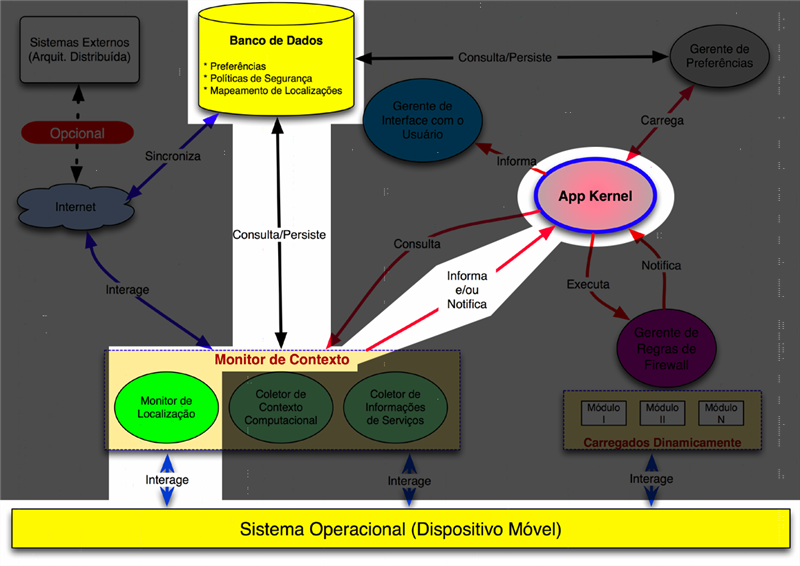
\includegraphics[width=0.80\textwidth]{../Pictures/Sequencias/Cenarios/CarregandoMetaDados_GPS/c1-2.png}
	\label{fig:c1-2}
\end{figure}

\end{frame}

\begin{frame}
\frametitle{\textbf Dispositivo M�vel \alert{com} GPS}
  \framesubtitle{Carregando Meta-Pol�ticas e Meta-Prefer�ncias}
  
\begin{figure}[htbp]
	\centering
		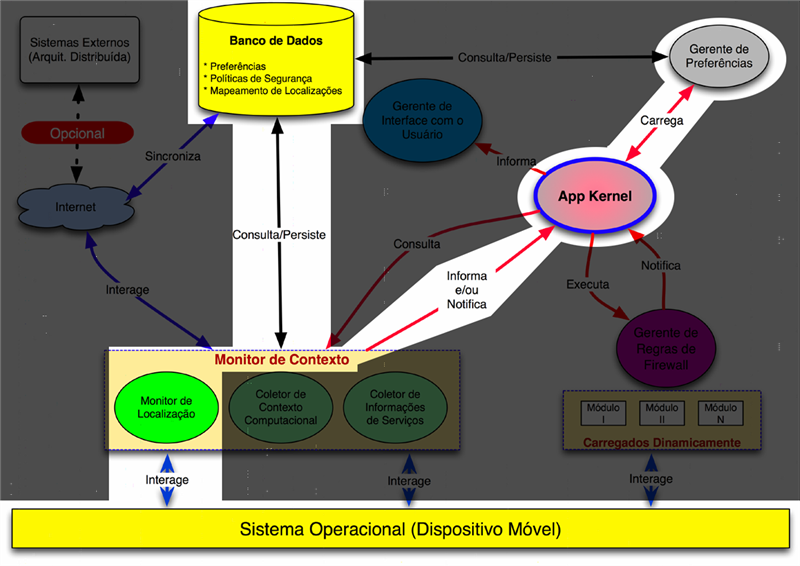
\includegraphics[width=0.80\textwidth]{../Pictures/Sequencias/Cenarios/CarregandoMetaDados_GPS/c1-3.png}
	\label{fig:c1-3}
\end{figure}

\end{frame}

\begin{frame}
  \frametitle{\textbf Dispositivo M�vel \alert{com} GPS}
  \framesubtitle{Carregando Meta-Pol�ticas e Meta-Prefer�ncias}

\begin{figure}[htbp]
	\centering
		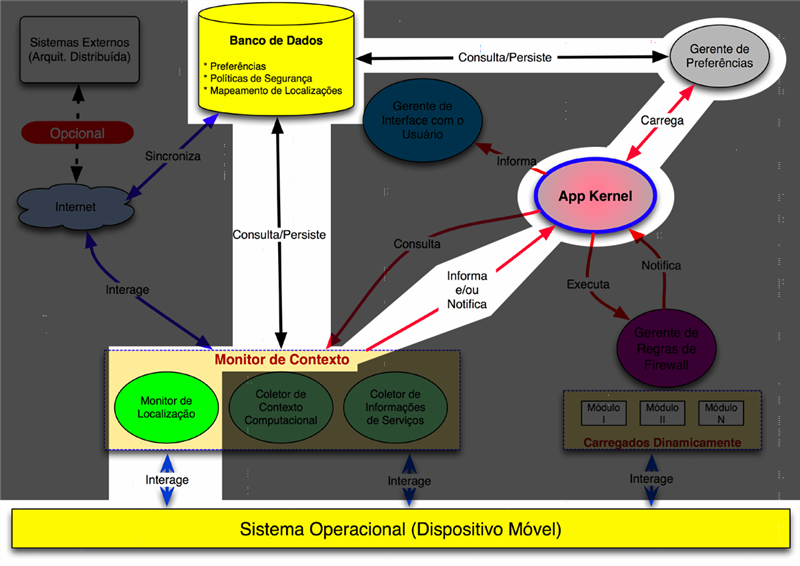
\includegraphics[width=0.80\textwidth]{../Pictures/Sequencias/Cenarios/CarregandoMetaDados_GPS/c1-4.png}
	\label{fig:c1-4}
\end{figure}

\end{frame}

\begin{frame}
  \frametitle{\textbf Dispositivo M�vel \alert{com} GPS}
  \framesubtitle{Carregando Meta-Pol�ticas e Meta-Prefer�ncias}

\begin{figure}[htbp]
	\centering
		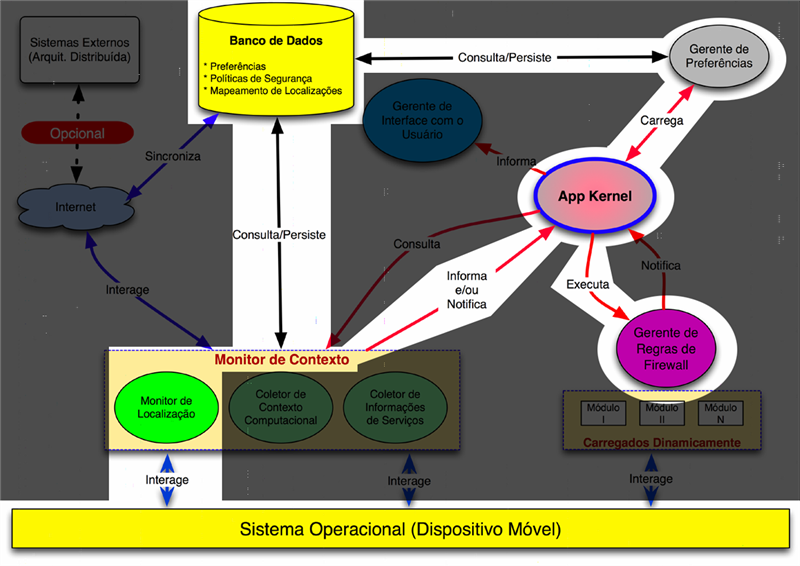
\includegraphics[width=0.80\textwidth]{../Pictures/Sequencias/Cenarios/CarregandoMetaDados_GPS/c1-5.png}
	\label{fig:c1-5}
\end{figure}

\end{frame}

\begin{frame}
  \frametitle{\textbf Dispositivo M�vel \alert{com} GPS}
  \framesubtitle{Carregando Meta-Pol�ticas e Meta-Prefer�ncias}

\begin{figure}[htbp]
	\centering
		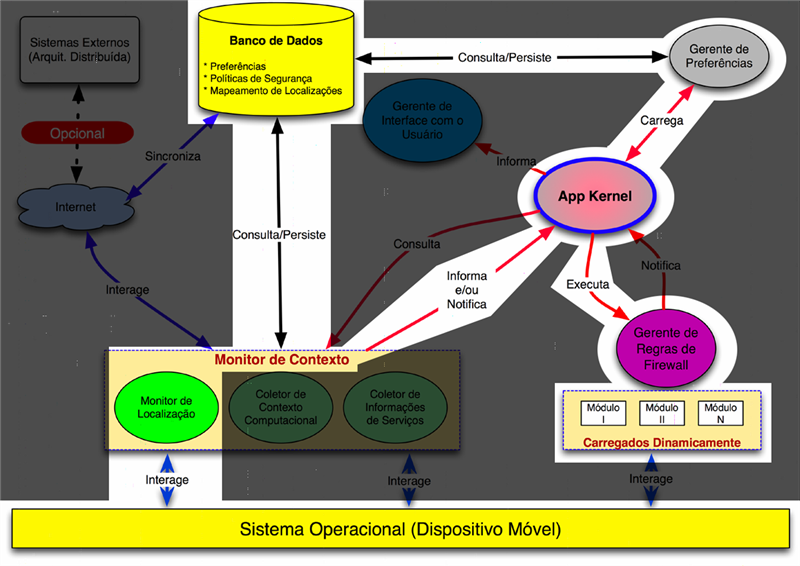
\includegraphics[width=0.80\textwidth]{../Pictures/Sequencias/Cenarios/CarregandoMetaDados_GPS/c1-6.png}
	\label{fig:c1-6}
\end{figure}

\end{frame}

\begin{frame}
  \frametitle{\textbf Dispositivo M�vel \alert{com} GPS}
  \framesubtitle{Carregando Meta-Pol�ticas e Meta-Prefer�ncias}

\begin{figure}[htbp]
	\centering
		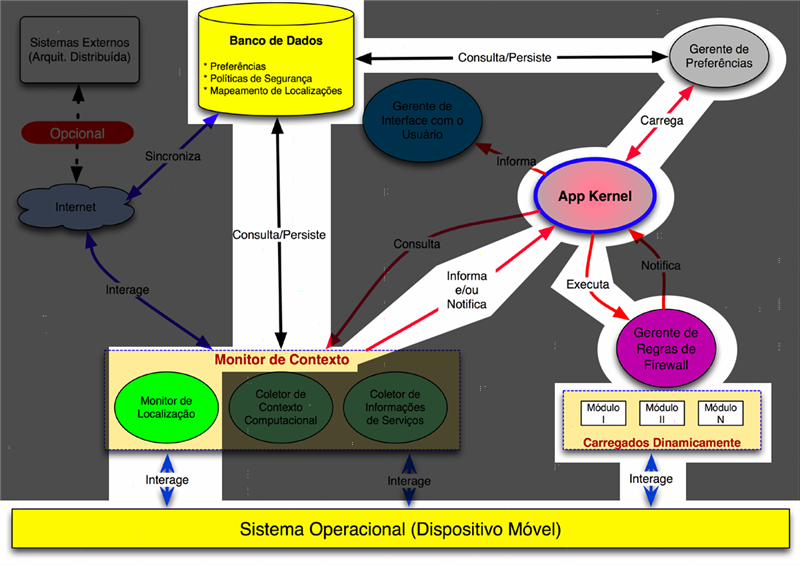
\includegraphics[width=0.80\textwidth]{../Pictures/Sequencias/Cenarios/CarregandoMetaDados_GPS/c1-7.png}
	\label{fig:c1-7}
\end{figure}

\end{frame}

\begin{frame}
  \frametitle{\textbf Dispositivo M�vel \alert{com} GPS}
  \framesubtitle{Carregando Meta-Pol�ticas e Meta-Prefer�ncias}

\begin{figure}[htbp]
	\centering
		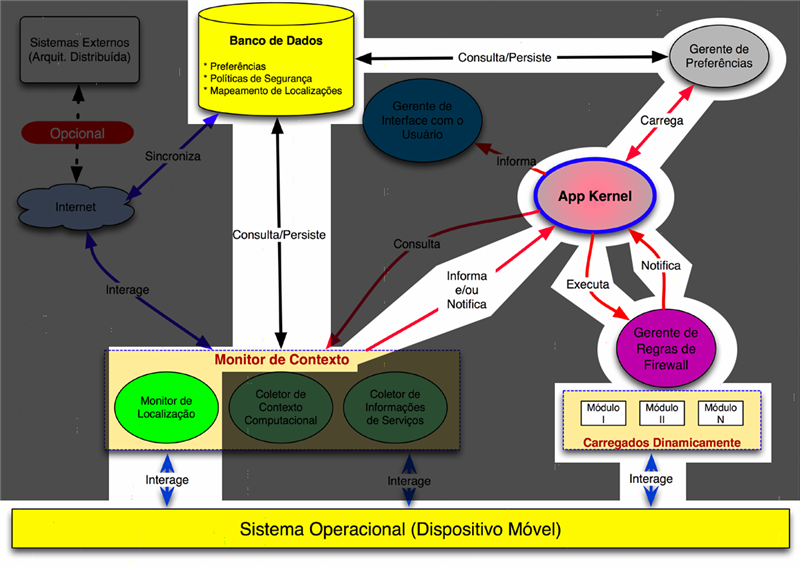
\includegraphics[width=0.80\textwidth]{../Pictures/Sequencias/Cenarios/CarregandoMetaDados_GPS/c1-8.png}
	\label{fig:c1-8}
\end{figure}

\end{frame}

\begin{frame}
  \frametitle{\textbf Dispositivo M�vel \alert{com} GPS}
  \framesubtitle{Carregando Meta-Pol�ticas e Meta-Prefer�ncias}

\begin{figure}[htbp]
	\centering
		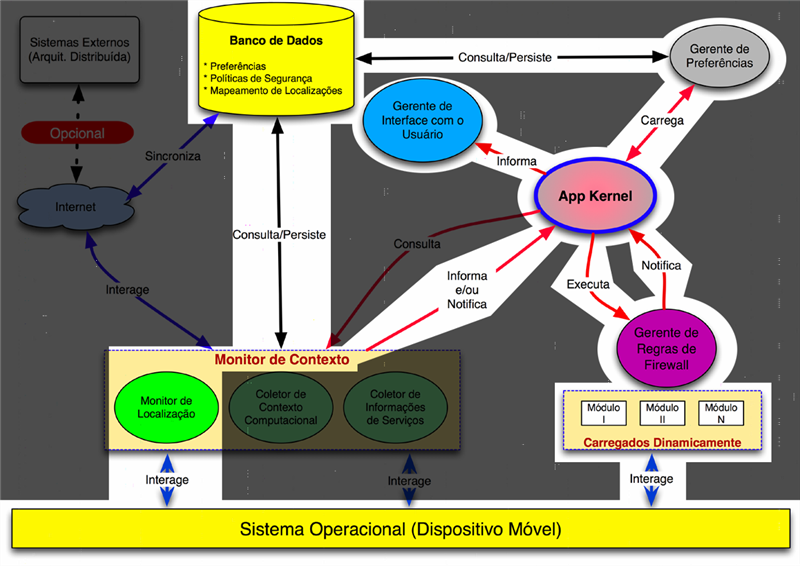
\includegraphics[width=0.80\textwidth]{../Pictures/Sequencias/Cenarios/CarregandoMetaDados_GPS/c1-9.png}
	\label{fig:c1-9}
\end{figure}

\end{frame}



%%%%%%%%%%%%%%%%%%%%%%%%%%%%%%%%%%%%%%%%%%%%%%%%%%%%%%%%%%%%%%%%%%%%%%%%%%%%%%%%%%%%%%%
%% Cen�rio 1 - Controlando Interfaces de Rede
%%%%%%%%%%%%%%%%%%%%%%%%%%%%%%%%%%%%%%%%%%%%%%%%%%%%%%%%%%%%%%%%%%%%%%%%%%%%%%%%%%%%%%%
\begin{frame}
  \frametitle{\textbf Controlando Interfaces de Rede}  

\begin{figure}[htbp]
	\centering
		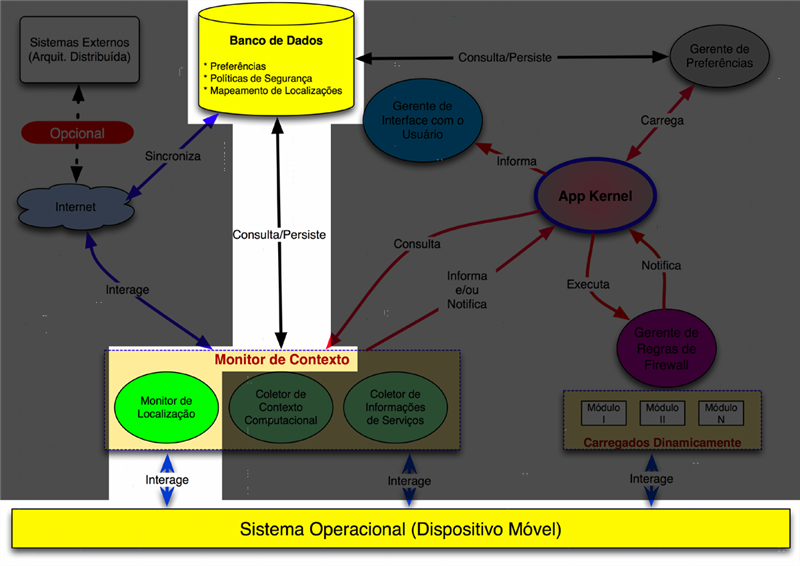
\includegraphics[width=0.80\textwidth]{../Pictures/Sequencias/Cenarios/ControlandoInterfaces/c2-1.png}
	\label{fig:c2-1}
\end{figure}

\end{frame}


\begin{frame}
  \frametitle{\textbf Controlando Interfaces de Rede}  

\begin{figure}[htbp]
	\centering
		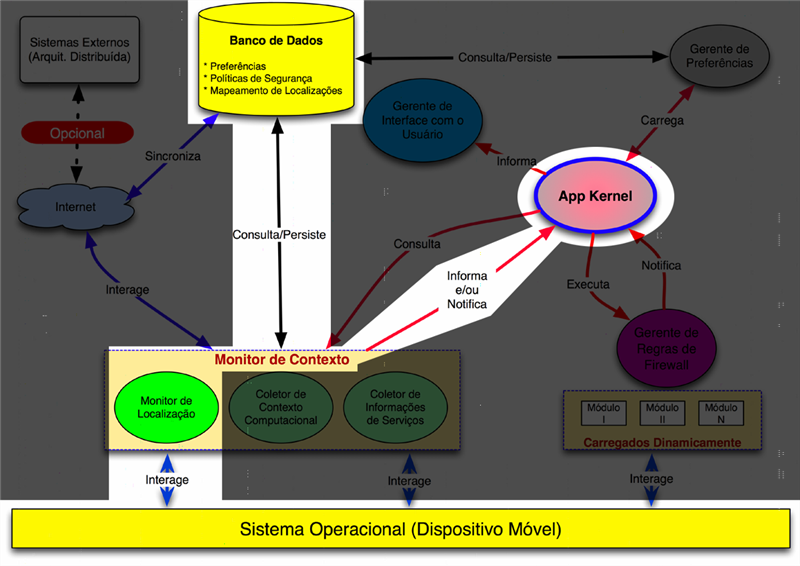
\includegraphics[width=0.80\textwidth]{../Pictures/Sequencias/Cenarios/ControlandoInterfaces/c2-2.png}
	\label{fig:c2-2}
\end{figure}

\end{frame}


\begin{frame}
  \frametitle{\textbf Controlando Interfaces de Rede}  

\begin{figure}[htbp]
	\centering
		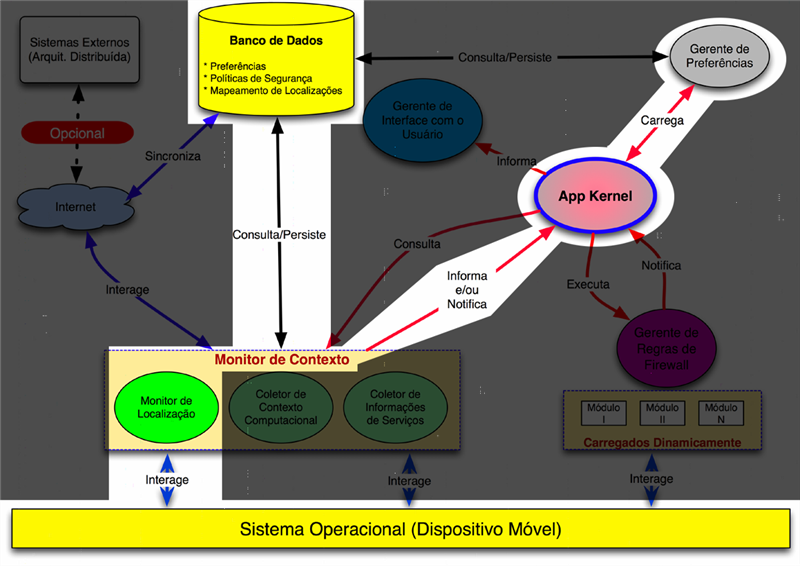
\includegraphics[width=0.80\textwidth]{../Pictures/Sequencias/Cenarios/ControlandoInterfaces/c2-3.png}
	\label{fig:c2-3}
\end{figure}

\end{frame}


\begin{frame}
  \frametitle{\textbf Controlando Interfaces de Rede}  

\begin{figure}[htbp]
	\centering
		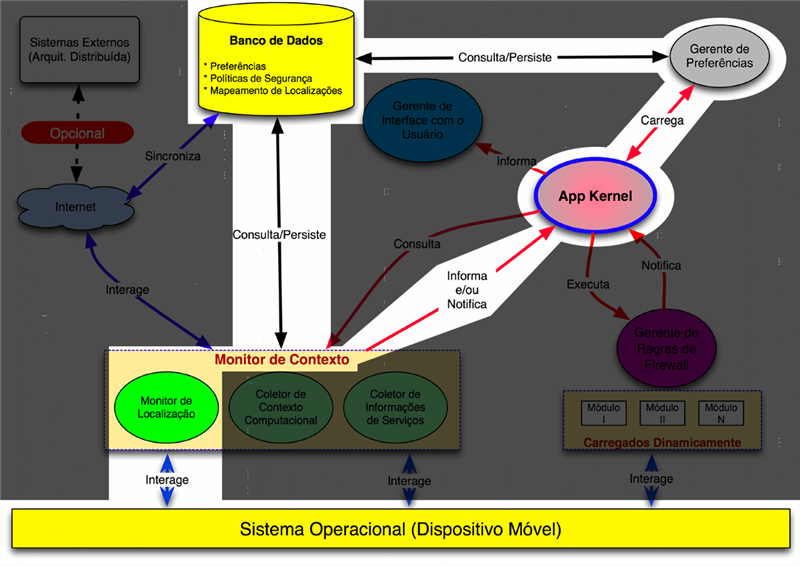
\includegraphics[width=0.80\textwidth]{../Pictures/Sequencias/Cenarios/ControlandoInterfaces/c2-4.png}
	\label{fig:c2-4}
\end{figure}

\end{frame}


\begin{frame}
  \frametitle{\textbf Controlando Interfaces de Rede}  

\begin{figure}[htbp]
	\centering
		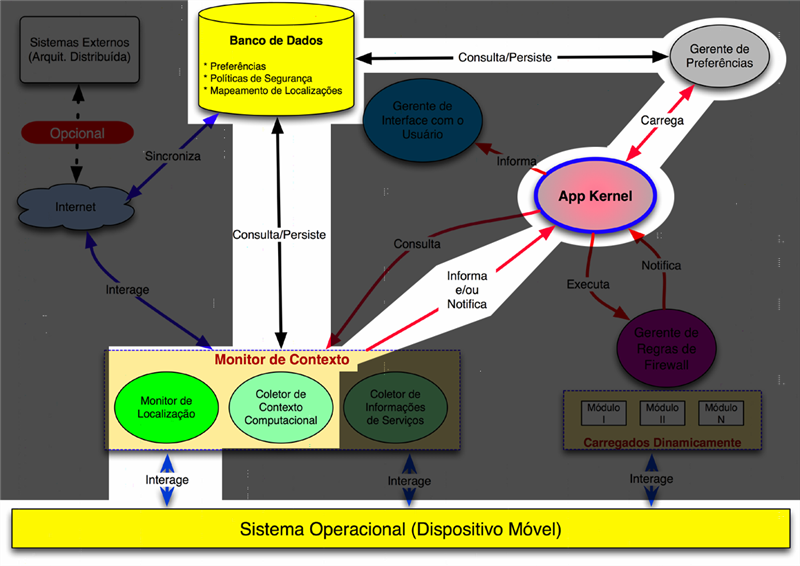
\includegraphics[width=0.80\textwidth]{../Pictures/Sequencias/Cenarios/ControlandoInterfaces/c2-5.png}
	\label{fig:c2-5}
\end{figure}

\end{frame}


\begin{frame}
  \frametitle{\textbf Controlando Interfaces de Rede}  

\begin{figure}[htbp]
	\centering
		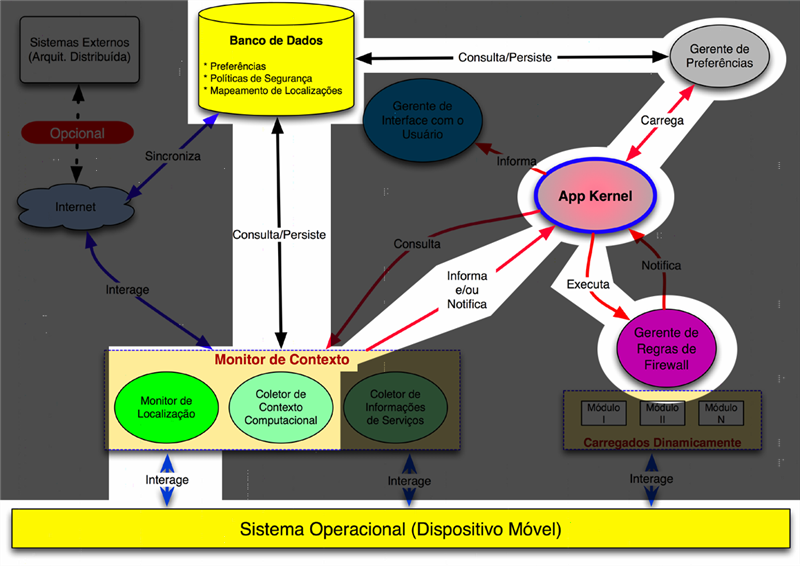
\includegraphics[width=0.80\textwidth]{../Pictures/Sequencias/Cenarios/ControlandoInterfaces/c2-6.png}
	\label{fig:c2-6}
\end{figure}

\end{frame}


\begin{frame}
  \frametitle{\textbf Controlando Interfaces de Rede}  

\begin{figure}[htbp]
	\centering
		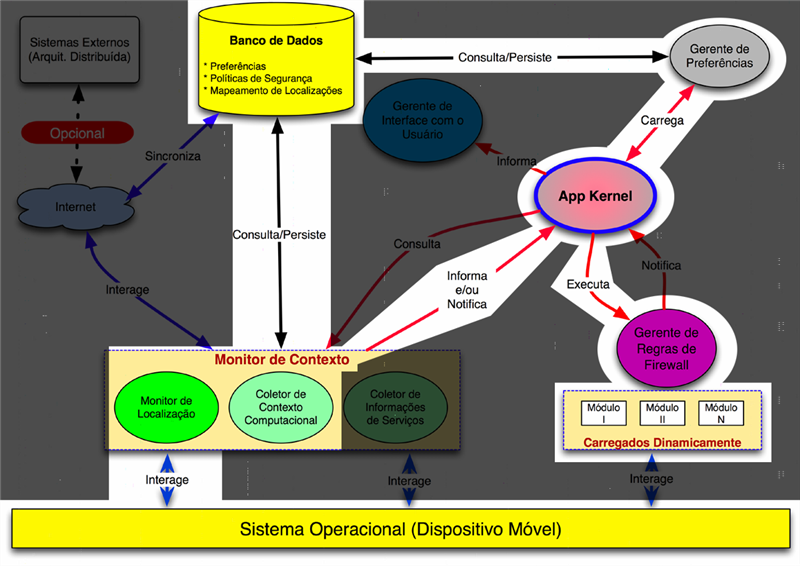
\includegraphics[width=0.80\textwidth]{../Pictures/Sequencias/Cenarios/ControlandoInterfaces/c2-7.png}
	\label{fig:c2-7}
\end{figure}

\end{frame}


\begin{frame}
  \frametitle{\textbf Controlando Interfaces de Rede}  

\begin{figure}[htbp]
	\centering
		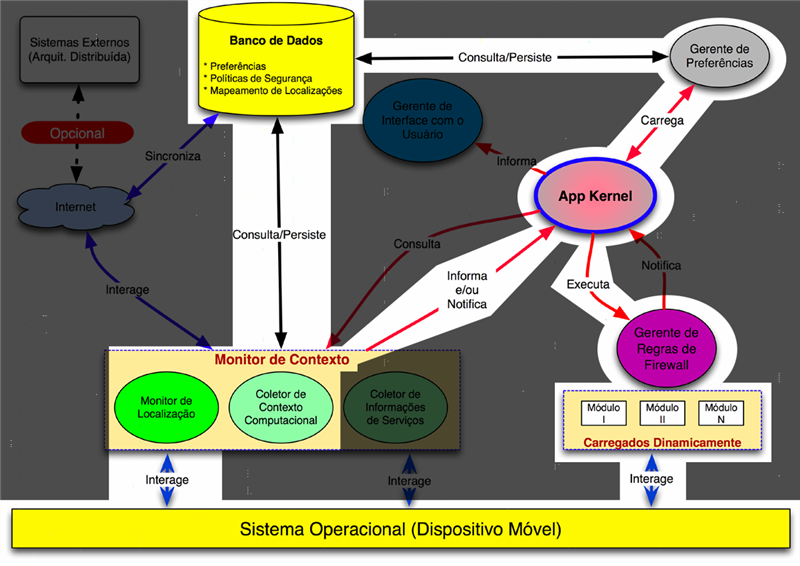
\includegraphics[width=0.80\textwidth]{../Pictures/Sequencias/Cenarios/ControlandoInterfaces/c2-8.png}
	\label{fig:c2-8}
\end{figure}

\end{frame}


\begin{frame}
  \frametitle{\textbf Controlando Interfaces de Rede}  

\begin{figure}[htbp]
	\centering
		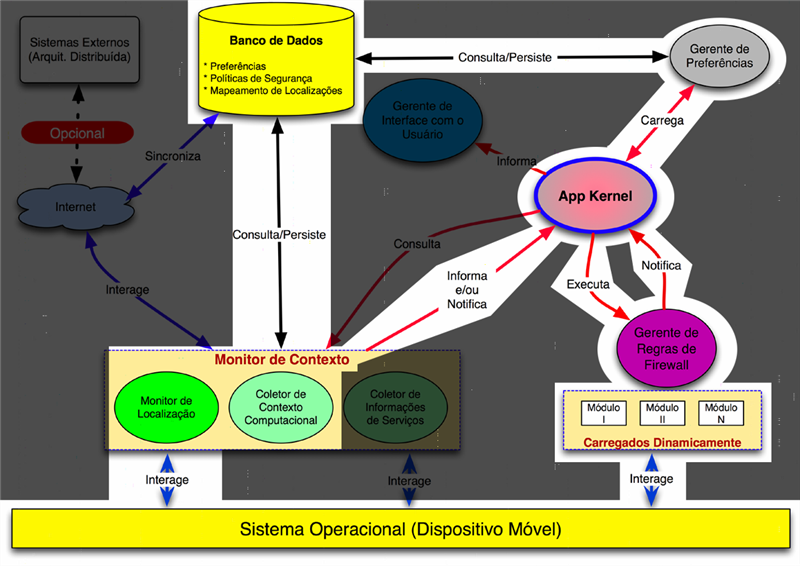
\includegraphics[width=0.80\textwidth]{../Pictures/Sequencias/Cenarios/ControlandoInterfaces/c2-9.png}
	\label{fig:c2-9}
\end{figure}

\end{frame}


\begin{frame}
  \frametitle{\textbf Controlando Interfaces de Rede}  

\begin{figure}[htbp]
	\centering
		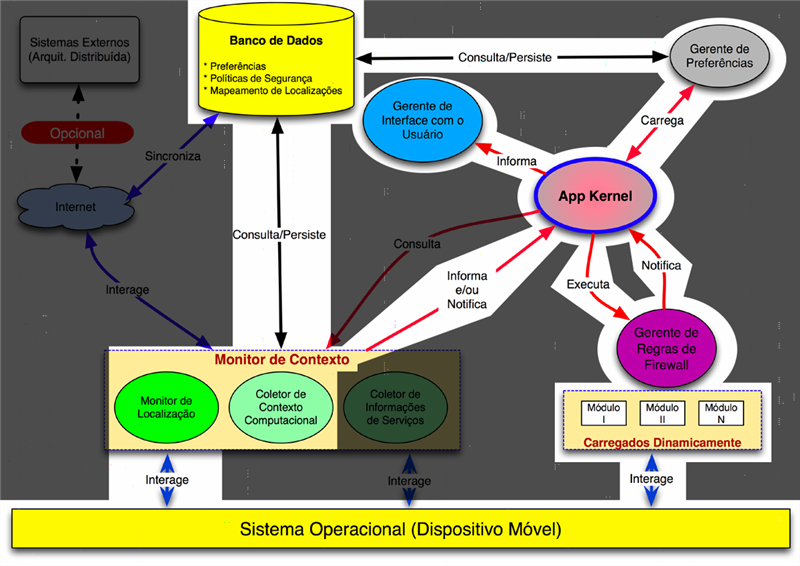
\includegraphics[width=0.80\textwidth]{../Pictures/Sequencias/Cenarios/ControlandoInterfaces/c2-10.png}
	\label{fig:c2-10}
\end{figure}

\end{frame}


%%%%%%%%%%%%%%%%%%%%%%%%%%%%%%%%%%%%%%%%%%%%%%%%%%%%%%%%%%%%%%%%%%%%%%%%%%%%%%%%%%%%%%%
%% Cen�rio 3 - Restringindo acessos entrantes e/ou saintes
%%%%%%%%%%%%%%%%%%%%%%%%%%%%%%%%%%%%%%%%%%%%%%%%%%%%%%%%%%%%%%%%%%%%%%%%%%%%%%%%%%%%%%%
\begin{frame}
  \frametitle{\textbf Restringindo acessos}  

\begin{figure}[htbp]
	\centering
		\includegraphics[width=0.80\textwidth]{../Pictures/Sequencias/Cenarios/ControlandoAcessos/c3-1.png}
	\label{fig:c3-1}
\end{figure}

\end{frame}


\begin{frame}
  \frametitle{\textbf Restringindo acessos}  

\begin{figure}[htbp]
	\centering
		\includegraphics[width=0.80\textwidth]{../Pictures/Sequencias/Cenarios/ControlandoAcessos/c3-2.png}
	\label{fig:c3-2}
\end{figure}

\end{frame}


\begin{frame}
  \frametitle{\textbf Restringindo acessos}  

\begin{figure}[htbp]
	\centering
		\includegraphics[width=0.80\textwidth]{../Pictures/Sequencias/Cenarios/ControlandoAcessos/c3-3.png}
	\label{fig:c3-3}
\end{figure}

\end{frame}


\begin{frame}
  \frametitle{\textbf Restringindo acessos}  

\begin{figure}[htbp]
	\centering
		\includegraphics[width=0.80\textwidth]{../Pictures/Sequencias/Cenarios/ControlandoAcessos/c3-4.png}
	\label{fig:c3-4}
\end{figure}

\end{frame}


\begin{frame}
  \frametitle{\textbf Restringindo acessos}  

\begin{figure}[htbp]
	\centering
		\includegraphics[width=0.80\textwidth]{../Pictures/Sequencias/Cenarios/ControlandoAcessos/c3-5.png}
	\label{fig:c3-5}
\end{figure}

\end{frame}


\begin{frame}
  \frametitle{\textbf Restringindo acessos}  

\begin{figure}[htbp]
	\centering
		\includegraphics[width=0.80\textwidth]{../Pictures/Sequencias/Cenarios/ControlandoAcessos/c3-6.png}
	\label{fig:c3-6}
\end{figure}

\end{frame}


\begin{frame}
  \frametitle{\textbf Restringindo acessos}  

\begin{figure}[htbp]
	\centering
		\includegraphics[width=0.80\textwidth]{../Pictures/Sequencias/Cenarios/ControlandoAcessos/c3-7.png}
	\label{fig:c3-7}
\end{figure}

\end{frame}


\begin{frame}
  \frametitle{\textbf Restringindo acessos}  

\begin{figure}[htbp]
	\centering
		\includegraphics[width=0.80\textwidth]{../Pictures/Sequencias/Cenarios/ControlandoAcessos/c3-8.png}
	\label{fig:c3-8}
\end{figure}

\end{frame}


\begin{frame}
  \frametitle{\textbf Restringindo acessos}  

\begin{figure}[htbp]
	\centering
		\includegraphics[width=0.80\textwidth]{../Pictures/Sequencias/Cenarios/ControlandoAcessos/c3-9.png}
	\label{fig:c3-9}
\end{figure}

\end{frame}


\begin{frame}
  \frametitle{\textbf Restringindo acessos}  

\begin{figure}[htbp]
	\centering
		\includegraphics[width=0.80\textwidth]{../Pictures/Sequencias/Cenarios/ControlandoAcessos/c3-10.png}
	\label{fig:c3-10}
\end{figure}

\end{frame}


\begin{frame}
  \frametitle{\textbf Restringindo acessos}  

\begin{figure}[htbp]
	\centering
		\includegraphics[width=0.80\textwidth]{../Pictures/Sequencias/Cenarios/ControlandoAcessos/c3-11.png}
	\label{fig:c3-11}
\end{figure}

\end{frame}


\begin{frame}
  \frametitle{\textbf Restringindo acessos}  

\begin{figure}[htbp]
	\centering
		\includegraphics[width=0.80\textwidth]{../Pictures/Sequencias/Cenarios/ControlandoAcessos/c3-12.png}
	\label{fig:c3-12}
\end{figure}

\end{frame}


%%%%%%%%%%%%%%%%%%%%%%%%%%%%%%%%%%%%%%%%%%%%%%%%%%%%%%%%%%%%%%%%%%%%%%%%%%%%%%%%%%%%%%%
%% Cen�rio 4 - Sincroniza��o Manual do Banco de Dados
%%%%%%%%%%%%%%%%%%%%%%%%%%%%%%%%%%%%%%%%%%%%%%%%%%%%%%%%%%%%%%%%%%%%%%%%%%%%%%%%%%%%%%%
\begin{frame}
  \frametitle{\textbf Sincroniza��o Manual do Banco de Dados}  

\begin{figure}[htbp]
	\centering
		\includegraphics[width=0.80\textwidth]{../Pictures/Sequencias/Cenarios/SincronizandoBancoManual/c4-1.png}
	\label{fig:c4-1}
\end{figure}

\end{frame}


\begin{frame}
  \frametitle{\textbf Sincroniza��o Manual do Banco de Dados}  

\begin{figure}[htbp]
	\centering
		\includegraphics[width=0.80\textwidth]{../Pictures/Sequencias/Cenarios/SincronizandoBancoManual/c4-2.png}
	\label{fig:c4-2}
\end{figure}

\end{frame}


\begin{frame}
  \frametitle{\textbf Sincroniza��o Manual do Banco de Dados}  

\begin{figure}[htbp]
	\centering
		\includegraphics[width=0.80\textwidth]{../Pictures/Sequencias/Cenarios/SincronizandoBancoManual/c4-3.png}
	\label{fig:c4-3}
\end{figure}

\end{frame}


\begin{frame}
  \frametitle{\textbf Sincroniza��o Manual do Banco de Dados}  

\begin{figure}[htbp]
	\centering
		\includegraphics[width=0.80\textwidth]{../Pictures/Sequencias/Cenarios/SincronizandoBancoManual/c4-4.png}
	\label{fig:c4-4}
\end{figure}

\end{frame}


\begin{frame}
  \frametitle{\textbf Sincroniza��o Manual do Banco de Dados}  

\begin{figure}[htbp]
	\centering
		\includegraphics[width=0.80\textwidth]{../Pictures/Sequencias/Cenarios/SincronizandoBancoManual/c4-5.png}
	\label{fig:c4-5}
\end{figure}

\end{frame}


\begin{frame}
  \frametitle{\textbf Sincroniza��o Manual do Banco de Dados}  

\begin{figure}[htbp]
	\centering
		\includegraphics[width=0.80\textwidth]{../Pictures/Sequencias/Cenarios/SincronizandoBancoManual/c4-6.png}
	\label{fig:c4-6}
\end{figure}

\end{frame}


\begin{frame}
  \frametitle{\textbf Sincroniza��o Manual do Banco de Dados}  

\begin{figure}[htbp]
	\centering
		\includegraphics[width=0.80\textwidth]{../Pictures/Sequencias/Cenarios/SincronizandoBancoManual/c4-7.png}
	\label{fig:c4-7}
\end{figure}

\end{frame}


\begin{frame}
  \frametitle{\textbf Sincroniza��o Manual do Banco de Dados}  

\begin{figure}[htbp]
	\centering
		\includegraphics[width=0.80\textwidth]{../Pictures/Sequencias/Cenarios/SincronizandoBancoManual/c4-8.png}
	\label{fig:c4-8}
\end{figure}

\end{frame}

\begin{frame}
  \frametitle{\textbf Sincroniza��o Manual do Banco de Dados}  

\begin{figure}[htbp]
	\centering
		\includegraphics[width=0.80\textwidth]{../Pictures/Sequencias/Cenarios/SincronizandoBancoManual/c4-9.png}
	\label{fig:c4-9}
\end{figure}

\end{frame}


%\section{Recomenda��es para Instala��o}

\subsection{Dispositivo M�vel}
\begin{frame}
		\frametitle{Recomenda��es para Instala��o}
		\framesubtitle{Dispositivo M�vel}

		
\begin{itemize}
	\item Para instalar o F�nix Firewall System no Dispositivo M�vel � necess�rio que:
			\begin{itemize}
				\item O Dispositivo m�vel possua \textbf{Sistema Operacional}.
				\item \textbf{Sistema Operacional} que possua recursos de filtragem de pacotes TCP/IP.
				\item \textbf{API} para utilizar os recursos de filtragem de pacotes.
				\item \textbf{API} para utilizar os recurso de Interface Gr�fica com o Usu�rio.
				\item \textbf{Interface} de rede 802.11 compat�vel.
				\item \textbf{Mem�ria} de armazenamento \textbf{dispon�vel} maior ou igual a 20Mb.
				\item \textbf{Processador} com freq��ncia superior a 100Mhz.
			\end{itemize}
\end{itemize}

\end{frame}

%_______________________________________________________________________
\subsection{Plataforma Distribu�da}
\begin{frame}
		\frametitle{Recomenda��es para Instala��o}
		\framesubtitle{Plataforma Distribu�da}

\begin{itemize}
	\item Para instalar a plataforma Distribu�da do F�nix Firewall System \textbf{(Opcional)}:
			\begin{itemize}
				\item \textbf{Sistema Operacional} que suporte Java.
				\item \textbf{Interface de rede} compat�vel com protocolo TCP/IP.
				\item \textbf{Banco de Dados} relacional compat�vel com SQL.
				\item \textbf{Endere�o IP} v�lido no dom�nio da Internet.
				\item \textbf{Dom�nio} v�lido registrado.				
				\item \textbf{Mem�ria} secund�ria \textbf{dispon�vel} maior ou igual a 100Mb.
				\item \textbf{Mem�ria} principal (RAM) maior ou igual a 512Mb. 
				\item \textbf{Processador} com freq��ncia superior a 600Mhz.
			\end{itemize}
\end{itemize}

\end{frame}
%\section{Desafios e Requisitos no Desenvolvimento e Uso}

\begin{frame}
	\frametitle{Desafios e Requisitos no Desenvolvimento e Uso}
			\begin{figure}[htbp]
				\centering
					\includegraphics[width=1.00\textwidth]{../Pictures/Baixa/Dispositivos.PNG}
				\label{fig:Dispositivos}
	\end{figure}
\end{frame}

\subsection{Recursos de Hardware}
\begin{frame}
  \frametitle{Desafios e Requisitos no Desenvolvimento e Uso}
  \framesubtitle{Recursos de Hardware}
				\begin{itemize}
					\item Tela reduzida.
					\item Entrada de dados limitada.
					\item Energia limitada.
				\end{itemize}
\end{frame}

%_______________________________________________________________________

\subsection{Recursos de Software}

\begin{frame}

  \frametitle{Desafios e Requisitos no Desenvolvimento e Uso}
  \framesubtitle{Recursos de Software}
				\begin{itemize}
					\item Sistemas Operacionais minimalistas.
					\item API�s limitadas.
					\item Pouca documenta��o para desenvolvimento de m�dio a baixo n�vel.					
				\end{itemize}
\end{frame}

%_______________________________________________________________________
\subsection{Interatividade com o usu�rio}
\begin{frame}
	\frametitle{Desafios e Requisitos no Desenvolvimento e Uso}
  \framesubtitle{Interatividade com o usu�rio.}
				\begin{itemize}
						\item Causa consumo de energia.
		  			\item Telas bem sucintas e informativas.
		  			\item Avisos e solicita��es intuitivas.
				\end{itemize}
\end{frame}

%_______________________________________________________________________
\subsection{Conectividade (Intermit�ncia)}
\begin{frame}
	\frametitle{Desafios e Requisitos no Desenvolvimento e Uso}
  \framesubtitle{Conectividade \textit{(Intermit�ncia)}.}
				\begin{itemize}
					\item Mobilidade.
					\item Largura de banda menor.
					\item Maior taxa de bits errados.
					\item Pagamento pelos servi�os.
				\end{itemize}
\end{frame}
\section{Nossa Contribui��o}

\begin{frame}
	\frametitle{Nossa Contribui��o}
  
		\begin{center}
				\LARGE Nossa principal contribui��o � o \textbf{Projeto Arquitetural de um Firewall Pessoal para Dispositivos M�veis}, que se utiliza do paradigma de localiza��o do usu�rio para carregar prefer�ncias e pol�ticas de seguran�a.
		\end{center}
		
\end{frame}


\begin{frame}[allowframebreaks]
	\frametitle{Nossa Contribui��o}
	  
				\begin{itemize}					
					\item \alert{\textbf{[SEGURAN�A]}} \\
					Aumentar o n�vel de seguran�a contra os ataques vindo da rede de comunica��o;
					\item \alert{\textbf{[CONTROLE]}} \\
					Controlar o acesso aos recursos do dispositivo m�vel e as informa��es;					
					\item \alert{\textbf{[POL�TICAS E PREFER�NCIAS]}} \\
					Flexibilidade para que o usu�rio execute, crie e edite suas prefer�ncias e pol�ticas de seguran�a;					
				\end{itemize}

\end{frame}	

	

\begin{frame}[allowframebreaks]
	\frametitle{Diferencial do F�nix Firewall System}

		\begin{itemize}
					\item \alert{\textbf{[LOCALIZA��O]}} \\
					Carregamento de Pol�ticas e Prefer�ncias baseado na localiza��o do usu�rio;
					\item \alert{\textbf{[INTERATIVIDADE CONTROLADA]}} \\
					N�vel de Interatividade controlada pelo usu�rio;
					\item \alert{\textbf{[META-POL�TICAS]}} \\
					Meta-pol�ticas export�veis;
					\item \alert{\textbf{[NOTIFICA��O]}} \\
					Servi�o de notifica��o do usu�rio via Web;					
		\end{itemize}

\end{frame}
\section{Trabalhos Futuros}

\begin{frame}
	\frametitle{Trabalhos Futuros}
	
			\begin{itemize}
					\item Implementar o recurso de \textbf{meta-pol�ticas} para outras plataformas de hardware (Ex.: Desktop, Tablet, Servidores etc);
					\item Integrar diferentes servi�os de localiza��o � Arquitetura Distribu�da (Ex.: RFID, Placelab, MoCA etc);
					\item Arquitetura distribu�da para detec��o de riscos e falhas de seguran�a (Ex.: CVE e CVSS);
					\item Arquitetura distribu�da extens�vel para trabalhos futuros(Detec��o de intrus�o, An�lise Inteligente etc);
			\end{itemize}

\end{frame}
% All of the following is optional and typically not needed. 
\appendix
\section<presentation>*{Bibliografia}

\begin{frame}[allowframebreaks]
  \frametitle<presentation>{Leituras Recomendadas}
    
  \begin{thebibliography}{10}
    
			  \beamertemplatebookbibitems
			  % Livros de Refer�ncia.
			
			  		 
			  \beamertemplatearticlebibitems
			  % Artigos de Refer�ncia.
			  	\bibitem{bellovin:1994}
			  			W.R. Bellovin, S.M.and Cheswick
			  			\newblock \emph{Network firewalls.}
							\newblock IEEE Communications Magazine, Vol. 32
			
			  	\bibitem{cvss:2008}
			  			FIRST (Forum of Incident Response and Security Teams)
			  			\newblock \emph{CVSS (Common Vulnerability Scoring System).}
							\newblock \url{http://www.first.org/cvss/}
			
					\bibitem{sage:2008}
							McAfee
							\newblock \emph{SAGE (Relat�rio Semestral de Seguran�a da McAfee). 2008.}
							\newblock \url{http://www.mcafee.com/us/local_content/reports/sage_2008.pdf}
							
					\bibitem{idc:2007}
							Instituto de Pesquisa IDC
							\newblock \emph{Brazil IT Investment Trends Insurance. 2007}
							\newblock \url{http://www.idclatin.com/}
			
			
				\beamertemplatearrowbibitems

					\bibitem{sms:2003}
							GSM 03.40
							\newblock \emph{Technical realization of the Short Message Service (SMS)}							
							\newblock \url{http://www.3gpp.org/ftp/Specs/html-info/0340.htm}

					\bibitem{durlacher:1999}
							Durlacher Researchs Ltd
							\newblock \emph{Mobile Commerce Report}
							\newblock \url{www.durlacher.com/research/res-reports.asp}

			
				\beamertemplatetextbibitems
				% Outras Refer�ncias

					\bibitem{snort:2008}
							Snort
							\newblock \emph{Open Source Network Intrusion Detector}
							\newblock \url{http://www.snort.org/}
					
					\bibitem{placelab:2008}
							Placelab
							\newblock \emph{A privacy-observant location system.}							
							\newblock \url{http://www.placelab.org/}

					\bibitem{moca:2008}
							Pontif�cia Universidade do Rio De Janeiro
							\newblock \emph{MoCA (Mobile Collaboration Architecture)}							
							\newblock \url{http://www.lac.inf.puc-rio.br/moca/}
						
					\bibitem{iPhone:2008}
							iPhone
							\newblock \emph{The iPhone}. Apple Inc.,2008.
							\newblock \url{http://en.wikipedia.org/wiki/IPhone}
											    
 
   \end{thebibliography}
\end{frame}

% Inclusao das secoes

\end{document}